
\chapter{Community detection}
\label{chap:community detection}
%\todo{Mpve spinglass to end}

This chapter moves to the next level of analysis, network communities, meso-scale structures in the network. Community detection is combined with  GSA (section~\ref{sec:Gene set tests}) to test if  PSP network communities are associated with intelligence or educational attainment. We will develop a general strategy to decide which community detection methods to use. 

Having discussed the genetics of differences in intelligence and educational attainment (section~\ref{sec:intelligence intro recent gwas}) and reviewed the insights gained from Gene Set Analysis (GSA) (section~\ref{sec:Gene set tests}) we can see that GSA provided evidences for the involvement of the brain, the synapse and neurogenesis as biological mechanisms that may underlie these traits\cite{hill2014functional},\cite{hill2019combined}. We also saw that GSA is limited by the choice of curated gene sets and it is hard to `discover' new gene sets. A prominent network orientated GSA methods paper called for data driven gene sets\cite{lamparter2016fast}. Given that the synaptic proteome is inherently modular (section~\ref{sec:intro large scale structure of networks from paper}) and the previous success of clustering algorithms in the synapse we test whether GSA and community detection can illuminate the genetics of intelligence as a paradigmatic case. 





\section{Network communities}
\label{sec: community detection intro gsa}


Communities, sub-graphs with dense interactions between community members and sparser connections to the rest of the graph (figure~\ref{fig:communities}), \cite{newman2012communities},\cite{fortunato2016community},\cite{girvan2002community} are the most well studied large-scale structure in networks\cite{newman2012communities}.  Absent from random graphs they are of interest because they may represent function units: in human and animal social networks they have been shown to correspond to real world groupings, and these assignments can be discovered using the pattern of connectivity of the vertices\cite{adamic2005political},\cite{zachary1977information}\cite{newman2018networks}\footnote{add page}.  An example of a community would be a group of friends in a social network; in the synaptic protein network, communities may represent functional modules\cite{pocklington2006proteomes},\cite{mclean2016improved} and could be used as data generated gene sets for competitive GSA.  

\begin{figure}
    \centering
    \includegraphics[width=\textwidth]{images/chapter_community_detection/creative_commons/F1large.jpg}
    \caption[Figure of three communities]{Line drawing of three communities showing dense connections within the communities (shaded) and fewer connections between communities}
    \tiny Creative commons for attribution see \url{https://commons.wikimedia.org/wiki/File:Network_Community_Structure.svg}
    \label{fig:communities}
\end{figure}

 Community detection methods when applied to smaller, earlier synaptic protein networks using over-representation GSA showed differential enrichment for disease and Gene Ontology terms in some communities\cite{pocklington2006proteomes},\cite{mclean2016improved}.  One study that used over representation GSA to test communities from protein-protein interaction networks used the results from GWA studies to add to the list of disease associated genes for seventy different disorders\cite{ghiassian2015disease}. Their analysis did not, however, use all the information available in summary GWAS statistics, the protein-protein interaction network was generated using evidence other than direct interaction (such as co-expression) and the network was not representative of the tissues affected by the diseases or traits under consideration\cite{ghiassian2015disease}.

Different tissues will contain different proteins and so the protein interaction network will have different nodes and edges. Vertex (node) statistics such as degree will be different and community detection algorithms may give different results.

The hierarchical divisive edge betweenness community detection method (Girvan–Newman algorithm) \cite{girvan2002community} has been used (section~\ref{sec:Newman and Girvan}) to discover communities in the protein-protein interaction graph of the NRC/MASC complex (248 edges, 105 nodes)\cite{pocklington2006proteomes}. This method has the advantage that the number of communities does not have to be determined in advance, the optimum level to stop the division is the maximum of an objective function, the modularity ($Q$), which determines the quality of the division of a network into communities\cite{girvan2002community}. 
%  Modularity had previously been introduced in the context of categorical assortativity.  Modularity is a measure of the difference between the number of edges found between members of a community and the expected number of edges given the degree of the network. In nominal assortativity\textcolor{red}{A} there were two groups, one that had the property and one that did not; an alternative way to see this is as two communities (cf adamcic). This is calculated using a random model of edge generation, the configuration model, where the degree of nodes is fixed and the edges assigned at random\cite{fortunato2016community}. 
 
\subsection{Modularity}
\label{sec:modularity introduction}
Modularity ($Q$) was used as a measure of nominal assortativity (equation~\ref{eq:categorical assortativity}, section~\ref{sec:assortativity}) the extent to which vertices that share a property are linked. A natural extension is as a measure of the quality of the division of the network into multiple groups, communities, where community membership is the property that nodes possess that maximises the modularity. 

 The most common method of community detection seek to maximise an objective function typically the modularity (see section~\ref{sec:modularity introduction} and Eq(\ref{eq: modularity A-kk delta group})) over possible partitions of the network to obtain non-overlapping groupings of the nodes\cite{newman2013spectral}. Alternately a statistical model can be used to find the community allocation most likely to generate the network although modularity and maximum likelihood approaches have been shown to be equivalent\cite{newman2016equivalence}. Modularity maximisation is computationally hard (NP complete\cite{brandes2007modularity}) and a number of heuristics have been described to provide approximations to the optimal modularity\cite{newman2013spectral}. Community detection algorithms also vary by being divisive or agglomerative and hierarchical (where smaller clusters are nested in larger ones) or partitional (where the best division of the network is sought without regard for hierarchy\cite{reichardt2006statistical}). 

 With increasing graph size some algorithms can become unstable, give rise to improbable community sizes, or become prohibitively computationally expensive\cite{pocklington2006proteomes},\cite{mclean2016improved}. 
McLean et al.\cite{mclean2016improved} described a parallelised implementation of the edge betweenness algorithm used previously on the NRC-MASC complex\cite{pocklington2006organization} and found it to be prohibitively slow with large networks. With a contemporary (2016) version of the human PSD proteome (V=1,312, E=8,031) the algorithm took 14 days (20,160 minutes) and the estimated completion time for a sequential implementation was 26 days (37,889 minutes). For all edge betweenness algorithms including parallelised implementations there is a steep inflection point in running time at around 4,000 edges (figure 1 in the manuscript\cite{mclean2016improved}).

One method of community detection that scales well with network size makes use of the spectral properties of the matrix representations of the network\cite{newman2013spectral}.  The network can be recurrently partitioned using the sign of the leading eigenvector of the modularity matrix\cite{newman2013spectral}.  McLean et al \cite{mclean2016improved} provide an implementation of this algorithm, which we will use in this chapter, along with the random walk and edge betweenness algorithms optimised for computers with multiple cores. Examining the performance of these algorithms on an earlier network model of the human post synaptic density (PSD) proteome (V=1,312, E=8,031) they found that the spectral clustering method with a fine-tuning step provided the best performance, measured by running time, community size and differential functional enrichment. 

In this chapter I will first try to find the best community detection algorithm for the larger (V=3,457) PSP. This will expand upon the analysis of McLean\cite{mclean2016improved} et al. as I will look in particular for algorithms that produce communities well suited for gene set analysis. The size of the communities generated is important as confounding effects can occur with large gene sets\cite{de2016statistical} and there may also be an optimum size of cohesive communities \cite{leskovec2009community}. On the other hand large numbers of small communities will result in sets dominated by the most significant genes and an increased penalty for multiple testing with a resultant decrease in power in analysing population GWAS-GSA. Algorithms that are prohibitively slow on networks of over 3000 nodes will not be suitable and algorithms that are `self-tuning', lacking additional parameters or the necessity to determine community size in advance, are preferred as they simplify study design. If there are not clear default or optimal parameters settings then each different setting could (should?) be regarded as a different test increasing type I error. 

Prospective algorithms in addition should be readily implementable and produce communities that `look right' and \textit{generally} correspond to functional units. 


\section{Communities}
\label{sec:alternate intro}

 Before testing communities using GSA we have to decide on an appropriate community detection algorithm or algorithms.

\subsection{Assessment of communities}
\label{sec:assessment of communities}
A number of benchmarks for community detection algorithms exist including the use of networks where we know the community allocation of the vertices (`Ground truth'\cite{yang2015defining}, examples include Zachary's Karate club\cite{zachary1977information}) or the use of benchmark networks which can be simple (Girvan-Newman, 128 nodes, four communities\cite{girvan2002community}) or derived from a more realistic generative model (Lancichinetti–Fortunato–Radicchi (LFR)\cite{lancichinetti2008benchmark}). Although they have been used to determine the `best' algorithm under different circumstances (\cite{yang2016comparative}) they have been less widely reported to select an algorithm for a particular the context of network analyses. The reason is probably that these analyses of algorithms\cite{yang2016comparative}, \cite{aldecoa2013exploring} are very involved but a simple procedure is to choose the LFR benchmark most similar to the network one is studying and assess algorithm performance on it in terms of performance measures and community size. 

Looking at the performance of community detection algorithms on ground truth communities Yang and Leskovec (2015) describe the usual process of assessing community detection performance. It bears quoting at length:

``Generally, after some community detection algorithm identifies communities based on the network structure, the essential next step is to interpret the communities by identifying a common external property or a function that the members of a given community share and around which the community organizes. \textit{For example, given a protein–protein interaction network of a cell, one first identifies communities based on the structure of the network and then examines that these communities correspond to real functional units of a cell}\cite{yang2015defining}\footnote{italics mine}.'' 

This has been the standard approach and has the obvious disadvantage that one only finds what one expects to find. In the example above one must \textit{know} the ``real functional units of the cell''. There is no chance to find new structure or organisation although it is well recognised that valuable structure can be discovered that differs from `ground truth'\cite{fortunato2016community}\footnote{p056104-8 para. 1; division of karate club into seven groups see also discussion of Girvan–Newman algorithm}. 

In studies of community detection in biological networks Gene Ontology definitions\cite{mclean2016improved}, Gene RIF, gene lists of gene disease associations (GDA) such as OMIM \cite{hamosh2005online}\footnote{(application \cite{ghiassian2015disease})}, ClinVar \cite{landrum2016clinvar}\footnote{application \cite{luck2020reference} ref 46}, CTD (Comparative Toxicogenomics Database) \cite{davis2019comparative}\footnote{application \cite{baker2012geneweaver}}, dbGAP \cite{tryka2014ncbi} DisGeNET \cite{pinero2020disgenet} \cite{pinero2016disgenet} and GWAS catalog\footnote{note to self -sic}\cite{welter2014nhgri} have been used  to assess whether the community detection algorithm is returning `natural' communities in the belief that a community enriched for these terms represents a functional unit, an entity that differs from a random selection of the elements that make up the network. 

There are a number of assumptions implicit in this including: that Gene Ontology or disease terms are precisely mapped, that a module has one function and that we know or can enumerate all functional units in a tissue (based on Gene Ontology or another repository).

One problem with this approach is that these lists of genes do not correspond closely with the findings of large scale population genetic studies. For example, in DisGeNET over 1,000 genes are associated with schizophrenia from curated sources and the total number of genes found in the database is 1,700\cite{pinero2020disgenet}. This represents approximately 8.5\% of protein encoding genes in the genome \cite{ezkurdia2014multiple}. This contrasts with 341 genes found in the Psychiatric Genomics Consortium–Schizophrenia Workgroup (PGC–SCZ) genome wide association study \cite{ripke2014biological}. These genes include those found in animal models or drug targets or may be found in diseases associated with schizophrenia. Using such a heterogenous group may lead to a set of genes with a limited connection to schizophrenia appearing to have a significantly enriched association.  

There is also the issue of the definition of disease.  DisGeNET disease refers to `actual diseases, disease symptoms and abnormal phenotypes that are observed as disease manifestations as well as normal traits and phenotypes that are currently explored in large scale Genome Wide Association studies (GWAS)\cite{pinero2020disgenet}'. Statements made about diseases and network topology such as where disease genes are within the interactome \cite{barabasi2016network},\cite{ghiassian2015disease} may refer to a number of different entities using Gene Disease Association. It may be better to limit a network analysis to a specific diseases or set of diseases and to differentiate between genetic variation associated the disease, gene expression in a specific phase of the disorder or other factors such as the genes targeted by common therapies. Finally all of the genes in these lists are scored equally in over-representation analyses whether they have a very strong association with the disorder or a weak one. Using information from GWA catalog to populate a gene disease association list does not provide the full polygenic signal from a group of genes found in summary GWA data. 

One way to test the assess clustering algorithms utility is to see whether they discovers communities that are associated with a disease or trait in population studies where the disease or trait is operationalised as much as possible (GWAS)\cite{cai2020reviewing}\cite{van2013power}. By using competitive Gene Set analysis using GWA study data as implemented in programs such as MAGMA\cite{de2015magma} or PASCAL\cite{lamparter2016fast} maximum information is retain from summary GWAS data and we  may also discover new insights into the subject of the GWA study.

We will still need some criteria to decide upon which algorithm to use in this GSA paradigm. Before turning to this we have to introduce the community detection methods. 





\section{Choice of community detection algorithm}
\label{sec:choice of community detection algorithm}
Given the number of community detection algorithms that are described it is likely none is optimal\cite{aldecoa2013exploring}. The Girvan-Newman (GN) benchmark \cite{girvan2002community} is a standardised benchmark with 128 nodes and four communities but is regarded as being too simple\cite{aldecoa2013exploring}. One limitation is that communities and degree are similar and the more demanding Lancichinetti–Fortunato–Radicchi (LFR)\cite{lancichinetti2008benchmark} allows scale free community size and degree(section~\ref{sec:LFR benchmark}). The other main way to assess algorithms is to compare communities with networks in which the `ground truth' (or metadata associated with the nodes) is known\footnote{leaving aside for now the question of what constitutes ground truth}\cite{leskovec2010empirical}.

Algorithms that perform well on small data sets often do not scale to larger networks\cite{girvan2002community},\cite{mclean2016improved},\cite{yang2016comparative}. In addition we would like to partition the network into communities that are both topologically robust but make sense biologically. It is hard to be prescriptive about what this means it is essentially to reject the implausible. For example, We have an intuition that the PSP network consists of more than three components, if it were divided by an algorithm into three components we would expect these would in turn have identifiable subdivisions. Biological plausibility\cite{pocklington2006organization} has been used to choose between algorithms and set parameters. At larger scale the best I can do is to reject the implausible or impracticable (see below). 

The goal of this chapter is to combined Gene set analysis (GSA) with community detection to provide data generated gene sets. GSA can be biased by very large and very small groups\cite{de2016statistical} and there are arguments that community sizes in real world networks tend to follow power law distributions (or at least heavily right skewed distributions)\cite{lancichinetti2008benchmark} or conform to an optimum size\cite{leskovec2010empirical}. A reasonable place to start would be community detection methods that give `good enough' communities on the PSP network. 


An ideal community detection algorithm would therefore

\begin{itemize}
    \item Perform well on standard benchmarks (LFR)
    \item Perform well on the PSP network \footnote{leaving aside what `well' is)}
    \item Have communities of `reasonable' size
    \item Have a reasonable run-time
    \item Have an available reliable implementation
    \item Not have a large number of parameters
\end{itemize}

The algorithms considered were those that are available in the widely used igraph package which have been previously used to measure algorithm performance \cite{yang2016comparative},\cite{de2014evaluating}.

\paragraph{Implementations}
The clustering of the PSP network used to provide gene sets to analyse the GWA study samples were performed by Dr. Colin McLean (see study design - section~\ref{sec:Study design topology based GSA}). The clustering to assess performance on benchmarks was carried out by me. I did not carry out Geodesic edge betweenness on the benchmark networks as the algorithm was already clearly impracticable and took a substantial amount of time to run on the ECDF (Edinburgh Compute and Data Facility) Linux Compute Cluster (Eddie) when performed on the PSP graph\footnote{\url{https://www.ed.ac.uk/information-services/research-support/research-computing/ecdf/high-performance-computing}}. Community detection on an earlier pilot study led to the decision to limit detection algorithms to those implemented in igraph or the CDM suite that had been developed within our group.  Markov clustering and the block stochastic inference were not carried out as part of the assessment of algorithms but after the initial analysis\footnote{they were not either implemented in igraph or developed `in house'. Markov clustering was assessed as it was used in ref \cite{ghiassian2015disease}. Block stochastic after an efficient implementation became available in graph tool\cite{peixoto_graph-tool_2014}.}.

\subsection{Girvan–Newman algorithm}
\label{sec:Newman and Girvan}
%\todo[inline]{newman and girvan or girvan and newman?}
Communities can be discovered by progressively removing links between dissimilar nodes. The Girvan–Newman algorithm\cite{girvan2002community} calculates the betweenness of all edges in the network. The edge with highest betweenness is then removed and the process is repeated. Over time the removal of these `bottleneck' edges breaks the network into highly connected subgraphs (divisive hierarchical community detection). The betweenness
needs to be recalculated at each stage and the optimum partition (the level in the dendrogram to stop dividing) is that which maximises modularity. This algorithm has been used to  to find
communities in the MASC complex\cite{pocklington2006proteomes}.

An implementation is provided in igraph but does not scale to networks of the scale of the PSP as it has complexity of $O(m^2n)$\cite{newman2004finding}. Even an efficient parallelised implementation took a prohibitively long time; for a network with 1108 nodes and 4691 edges on a single core the algorithm took 9690 minutes (approximately 6.7 days)\cite{mclean2016improved}.

%\todo[inline]{community induced graph in igraph cluster graph see url below}
%\url{https://igraph.org/python/doc/igraph.clustering.VertexClustering-class.html#cluster_graph}





\subsection{Spectral clustering}
Graphs can be divided into communities using the spectrum of the eigenvalues and eigenvectors of the matrices that represent them\cite{newman2006finding}. Spectral methods have been described for modularity maximisation, statistical inference and normalised graph cut partitioning and have been shown to be equivalent \footnote{at least in the case of two groups}\cite{newman2013spectral}.

Community allocation is assigned on the basis of the sign of the principal eigenvector of the modularity matrix (or the second eigenvector of the Laplacian). Spectral community detection with a fine tuning step was implemented using the CDM suite provided by the first author of \cite{mclean2016improved}. The theory underlying spectral clustering can be found in \cite{newman2013spectral} and supplemental section~\ref{sec:Spectral methods description}. Details of the implementation and fine tuning step can be found in McLean et al.\cite{mclean2016improved}. The C++ implementation is provided in the supplementary material. 


\subsection{Louvain}
\label{sec:Louvain}
The Louvain method,the university of the authors of the original paper. is a hierarchical agglomerative community detection method using modularity maximisation as the objective function. It functions very well at extreme scale and is fast\cite{blondel2008fast}.

The algorithm works by first assigning nodes into communities. Then those communities are in turn combined into communities composed of communities. The process stops when maximal modularity is achieved. It alternatively referred to as multilevel (see for example\cite{yang2016comparative}).
\subsubsection{Methods}

Louvain community detection was carried out using igraph Version 1.2.4.2 using the \texttt{cluster\_louvain} command. The Louvain implementation requires no parameters to be supplied other than an optional weights argument for weighted networks and this simplifies study design. The igraph implementation returns communities discovered at the level of hierarchy that maximises the modularity. The communities objects returned by the \texttt{cluster\_louvain} method were stored as vertex attributes in a .gml file provided by Dr C.McLean and converted into a .gmt file (GSA input file) using a custom R script\footnote{\url{source('~/RProjects/paper_xls_output/R/magma_synapse/make_synapse_gmt.R')}}. This procedure was used for all of the algorithms that were used to provide gene sets for GSA. 

\subsection{Infomap}
\label{sec:Infomap}

Infomap, described by Rosvall, is one of many algorithms conceptually based on the properties of a random walk across as network\cite{rosvall2008maps}. In such a random walk the walker will tend to remain in communities once in them (see also walktrap section~\ref{sec:walktrap}). Infomap uses information theory to find an optimal community structure and aims to minimise the descriptive length of an encoding of the community struture. The hypothetical random walk is given a binary encoding with movements in and out of communities given specific codes and movement within communities given codes. These do not have to be unique because the information already provided about the location in the walk can identify where the walk is in terms of a node or community. The goal is then to encode community entry and exit in such a way to minimise the descriptive length. The traversal of the actual community structure will be best described with a labelling that corresponds as close as possible to the community structure but there is also a cost to intra group movement and a tendency to produce shorter labels. Infomap was implemented using igraph for R with default arguments (n.b trials=10) as increasing the number of trials only led to a minimal increase in the modularity. 

% Gene set analysis of the ducational ability and intelligence GWA were carried out using MAGMA as described above \todo{add cross ref}. 
% \cite{blondel2008fast}
\subsection{Spinglass}
\label{sec:spinglass}

Community detection can be formulated as the solution of an infinite Potts spin glass where each node is coupled and the spin of each node in the ground state corresponds to the community. The Hamiltonian is minimised using simulated annealing\cite{kirkpatrick1983optimization}.  The energy of the ground state can be interpreted as a quality function. 

The parameter $\gamma$ which controls the balance between present and missing edges can also control the size of communities and their nesting eg with communities in higher gamma domains being nested within those in lower (see Reichardt\cite{reichardt2006statistical}). With $\gamma$=1 the solution should be similar to maximising the modularity\cite{eaton2012spin}.

There are a number of tunable parameters for the implementation of the spinglass algorithm implementation in igraph in addition to $\gamma$ there are: spins (default 25 - upper limit for number of communities); starting, stopping and cooling temperatures and update rules. 

\subsection{Walktrap}
\label{sec:walktrap}
The walk trap algorithm is an agglomerative community detection algorithm uses the properties of random walks to define distances between nodes and discover communities. At the stationary distribution the probability of being on a node is proportional to its degree. At earlier times nodes within communities are more likely to be visited by a random walk originating within that community. Short random walks (the default in igraph is four) should therefore stay in the community. The algorithm determines the random walk probability density scaled by the node degree\cite{pons2005computing}. The  The optimum level to stop merging the dendrogram is modularity by default in igraph. It has computational complexity of $O(n^3)$\cite{danon2005comparing} or $O(n^2 logn)$ on a sparse network\cite{yang2016comparative}.

\subsection{Fast greedy}
The fast greedy algorithm (abbreviated as fc) implemented in igraph is the Clauset Newman Moore (CNM) algorithm\footnote{\url{https://igraph.org/r/doc/cluster_fast_greedy.html}} and is a hierarchical agglomerative algorithm. Communities are merged if the merge results in the greatest gain in modularity\cite{clauset2004finding}. The algorithm starts with each node in a single community and achieves efficiency by updating a matrix of $\Delta Q_{ij}$ the change in modularity when communities $i$ and $j$ are merged. Its worst case running time is $O(md$ log$ n)$ where $m$ and $n$ are the number of vertices and edges as before and $d$ is the depth of the dendrogram representing the merges of communities. 

\subsection{Label propogation}
\label{sec:label propogation}
This heuristic algorithm runs in near linear time but has no guarantee that a similar clustering will be found (to a greater extent than other algorithms). In the implementation in igraph for R and python very disparate values of the modularity are found and often the modularity is very low\cite{raghavan2007near}. Each time the function is called in igraph for Python the modularity of the division is usually close to 0 although some are higher. With a number of iterations and keeping the partition with the highest modularity and acceptable division is achieved. 

The label propagation method is somewhat similar to algorithms such as $k$ nearest neighbours and $k$ means clustering. At the start each node belongs to a community consisting entirely of that node. In each round of the algorithm the label changes to that of the majority of its neighbours. Ties are broken. The method performs well on the LFR benchmarks see table~\ref{tab:benchmark LFR size 1000}.

\subsection{Markov Cluster Algorithm}
\label{sec:markov clustering}
The Markov Cluster Algorithm (MCL) is also conceptually based on random walks over the network with alternating patterns of expansion and contraction. After loops have been added the network is rendered as a stochastic matrix where the transition probability between two nodes of length $n$ is the stochastic matrix raised to the $n$th power. Vertices in similar communities should have a high probability of transitioning to one another and this effect is made more pronounced by contraction which does something. Markov clustering was implemented using the default command line arguments of Version 14.137 running on Ubuntu 16.04 (from \url{https://micans.org/mcl/})\cite{dongen2000graph}.


\subsection{Leading eigenvector community detection - LEC}
\label{sec:Leading eigenvector method}
A simple implementation of the leading eigenvector algorithm of Newman is provided as part of igraph. The principal difference between this and the spectral method implemented by McLean et al. is that there is no fine tuning step (there are also a number of differences in the calculation of the eigenvalue spectrum (see \cite{mclean2016improved}).  




\subsection{Stochastic block model}
\label{sec:stochastic block model}
The stochastic block model is a generative model of network and community structure that can incorporate both community structure and other features such as core periphery structure. It assumes that the network is generated from a set of group assignments $g$ and a matrix of probabilities $P$ where $P_{i,j}$ is the probability of an edge between two nodes if the nodes are in group $i$ and $j$. The likelihood of the partition is the product of the likelihood of each edge given the community structure. To find the best community structure the minimises the descriptive length of the community structure using an agglomerative heuristic and Monte Carlo sampling \cite{peixoto2014efficient}.

Stochastic block model inference was implemented using graph tool 2.37 for python\cite{peixoto_graph-tool_2014}. 






 \section{Lancichinetti–Fortunato–Radicchi (LFR) benchmark}
\label{sec:LFR benchmark}


The Lancichinetti–Fortunato–Radicchi (LFR) benchmark\cite{lancichinetti2008benchmark} generates a network with a degree  and community size distribution parameterised as a power law distribution\cite{lancichinetti2009community}  to accord with  their observed prevalence in real world networks (see \cite{radicchi2004defining},\cite{palla2005uncovering}). It is intended to be more challenging than the Girvan-Newman (GN) model which uses four communities\cite{girvan2002community}. A mixing parameter $\mu$, the proportion of edges found between communities, controls the amount of noise in the network and hence the difficulty of the task for the community detection algorithm. With increasing values of $\mu$ the modularity of the ground truth partition decreases (figure~\ref{fig:modularity_and_mu}).




\begin{figure}
    \centering
    \includegraphics[width=0.9\textwidth]{images/chapter_community_detection/ggplot2/LFR/Rplot_muandq_theme.png}
    \caption[Modularity and $\mu$ for LFR benchmark]{Plot of modularity with parameter $mu$ in LFR benchmark. Using LFR 3457 40617 benchmark}
    \tiny Plot \url{source('~/RProjects/fortunato/R/plot/new_plot_qandmu.R')}
    \tiny Calculations \url{/home/grant/Projects_/Python/src/Qandmu.ipynb}
    \label{fig:modularity_and_mu}
\end{figure}

% \subsubsection{Testing}
% Infomap and louvain do very well on lfr but spectral not so well. Infomap does perfectly with nmi but poorly with real world network. 
% settings = \url{g2= nx.generators.LFR_benchmark_graph(n=graph_n, tau1=3, tau2=1.1, mu=0.1, average_degree=10, max_degree=50, min_community=10,max_community=50, seed=1)}

% Set seed 1 See table~\ref{tab:benchmark LFR size 1000}

% \begin{table}[h]
%     \centering
%     \begin{tabular}{ll}
%     \toprule
%      Method    & NMI  \\
%      \midrule
%     Louvain     & 0.970\\
%     Infomap     & 1\\
%     Spectral & 0.949\\
%     Greedy & 0.873\\
%     Leading eigenvector & 0.620\\
%     Label propogation & 0.997\\
%     Out walk trap & 0.995\\
%     \bottomrule
%     \end{tabular}
%     \caption{Benchmark LFR size 1000. Generated using networkx for python}
%     \label{tab:benchmark LFR size 1000}
% \end{table}
% % Louvain =  0.9705355030878491

% % Info = 1 

% % Spec = 0.9486340326647721

% % Greedy = 0.8736469937608322

% % Leading eigenvector method igraph = 0.6202572106629003

% % Label propogation = 0.9966685735031502

% % Out walk trap = 0.9952730301593156

% its all the small or zero groups that give good nmi as the number of correctly misclassified is right so long as vertices a and b if in different groups are in different groups 
\subsubsection{Methods}
\label{sec:LFT methods}
The LFR benchmark networks were generated using the Python package NetworkX (version 2.4)\cite{hagberg2008exploring}. The NetworkX implementation is almost identical to the authors implementation\footnote{the differences are that rewiring is done at the end which is held to be equivalent and the community allocation is treated as an integer}. In addition to the power law exponent of the degree distribution either the minimum or average degree can be provided as arguments to generate the desired degree distribution\footnote{\tiny\url{https://networkx.org/documentation/networkx-2.1/reference/algorithms/generated/networkx.algorithms.community.community_generators.LFR_benchmark_graph.html}}.

The algorithm does not converge for all values of parameters and the distribution of values of $\mu$ obtained (figure 3 in\cite{lancichinetti2008benchmark}) is bi-modal distribution with peaks $P(\mu$) around 0.1 and 0.5\footnote{The authors of the NetworkX method note that `a somewhat narrower parameter set is likely to successfully produce a graph' which has also been my experience}.

Using the default parameter values of the authors' implementation resulted in a network where it was difficult to discriminate between algorithms even at $\mu=0.5$ as performance was almost universally good. 

Setting the minimum and maximum degree using the matching values of the PSP and degree exponent of 2.51 (section~\ref{sec:results degree distribution}) produces a network with  roughly equal vertices and edges (V:3,457, E:4,736), a mean degree of 2.74, and maximum degree 119 (degree assortativity -0.09, global transitivity 0.012). This is clearly a poor model for the PSP.

If instead, using the same degree exponent, one sets the mean degree parameter equal to the PSP mean (rather than setting minimum or maximum degree) the network is much more like the PSP although there are no nodes of degree less than seven . These make up 1,445 vertices of the PSP graph equivalent to 41.7\% of the vertices. This may be because the power law distribution does not hold in the low degree region of the degree distribution. This LFR benchmark network has 3,457 nodes and 40,617 edges.
The modularity was 0.431 for ground truth community allocations ($\mu$=0.375). The graph is available in .gml format\footnote{\url{git@github.com:14760/ipynotebooks_phd.git}}.

I have used an LFR benchmark close to the PSP as algorithms performance is known to vary depending on parameters such as network size and average degree\cite{wang2017comparison}.

The Potts model\cite{reichardt2004detecting} and modularity optimisation by simulated annealing\cite{guimera2004modularity} were assessed in the paper introducing the LFR benchmark\cite{lancichinetti2008benchmark}. The Louvain and Infomap algorithms were shown to perform best out of a number of algorithms on the LFR benchmark in a subsequent paper\cite{lancichinetti2009community}. A variety of spectral method was assessed on this occasion, the method of Donnetti and Munoz, which assigns nodes to clusters based on their proximity in an embedding in Euclidean space using a few of the eigenvectors of the Laplacian matrix\cite{donetti2004detecting}. The networks produced using the parameters from this paper\cite{lancichinetti2009community} are quite dissimilar to the PSP\footnote{\tiny the average degree is 20, the maximum degree 50, the exponent of the degree distribution is -2 and that of the community size distribution is -1.'\cite{lancichinetti2009community}}.
 The LFR benchmark has limitations, in addition to the difficulty in generated particular networks it is known to produce similar sized communities which differ from  real world networks\cite{orman2013towards},\cite{aldecoa2013exploring}. 

Networks generated using the LFR benchmark have been reported to have low transitivity and zero degree correlation in common with many other generative models and so do not completely capture the structure of complex networks \cite{orman2013towards},\cite{orman2009comparison}. However using the `PSP like' LFR network it is interesting to note the degree assortativity is $r$=-0.16  (PSP $r$=-0.18) table~\ref{Table:DegreeAssortativityNewman}) and the transitivity $C$=0.0415  (PSP=0.067 section~\ref{sec:results_global_clustering_coefficient}) and  $C_{WS}$ =0.0810\footnote{\tiny Code to generate LFR benchmark at\url{/home/grant/Projects_/Python/venvs/Create_LFR_similar_to_PSP.ipynb}}.

Given these limitations of the LFR benchmark, I have also used the performance of algorithms on the PSP, as measured by modularity and plausibility of group size, to determine the most appropriate algorithms to use. 


\paragraph{Measuring performance}
Normalised mutual information (NMI), derived from information theory, has been used as a measure of the quality of partitions of a network\cite{danon2005comparing} and lies in the range 0-1. The algorithms were assessed on the LFR benchmark by comparing the detected communities to the ground truth partition using the \url{compare_communities} method in igraph for Python. The mutual information, adjusted for the expected value of the mutual information (adjusted NMI)\cite{vinh2010information}, was calculated using scikit-learn\cite{abraham2014machine}. Normalised mutual information may not accurately reflect performance when there are a large number of communities\cite{amelio2015normalized},\cite{fortunato2016community}.


Normalised and adjusted normalised mutual information were  used to compare the similarity of the communities discovered in the PSP. Here the communities found by different algorithms are compared against one another rather than ground truth. 




% \textcolor{red}{This is bollocks}For a degree structure similar to the PSP it proved impossible to generate a community structure with a power exponent greater than 1.156 in the network x implementation of the LFR benchmarks using 1000 iterations (parameters - average degree 27, min\_community=20) .  Increasing minimum community size to 50 allowed a maximum $\beta$ of 1.6.\textcolor{red}{end}






% \subsubsection{Testing}
% Infomap and louvain do very well on lfr but spectral not so well. Infomap does perfectly with nmi but poorly with real world network. 
% settings = \url{g2= nx.generators.LFR_benchmark_graph(n=graph_n, tau1=3, tau2=1.1, mu=0.1, average_degree=10, max_degree=50, min_community=10,max_community=50, seed=1)}

% Set seed 1 See table~\ref{tab:benchmark LFR size 1000}

% \begin{table}[h]
%     \centering
%     \begin{tabular}{ll}
%     \toprule
%      Method    & NMI  \\
%      \midrule
%     Louvain     & 0.970\\
%     Infomap     & 1\\
%     Spectral & 0.949\\
%     Greedy & 0.873\\
%     Leading eigenvector & 0.620\\
%     Label propogation & 0.997\\
%     Out walk trap & 0.995\\
%     \bottomrule
%     \end{tabular}
%     \caption{Benchmark LFR size 1000. Generated using networkx for python}
%     \label{tab:benchmark LFR size 1000}
% \end{table}
% % Louvain =  0.9705355030878491

% % Info = 1 

% % Spec = 0.9486340326647721

% % Greedy = 0.8736469937608322

% % Leading eigenvector method igraph = 0.6202572106629003

% % Label propogation = 0.9966685735031502

% % Out walk trap = 0.9952730301593156

% its all the small or zero groups that give good nmi as the number of correctly misclassified is right so long as vertices a and b if in different groups are in different groups 


\subsubsection{LFR Performance}
\label{sec:lfrbm}
The performance of the igraph community detection algorithms, Markov Cluster algorithm and the Spectral Clustering Algorithm (CDM)\cite{mclean2016improved} on the LFR (PSP like) benchmark graph are shown in table~\ref{tab:Modularity, NMI and adjusted NMI on the LFR Benchmark PSPlike1}. A sizeable difference is seen between the NMI and Adjusted NMI, particularly for the Markov Clustering partition (NMI=0.653, Adj NMI=0.295), supporting the utility of including this measure\cite{vinh2010information}. 


\begin{table}[ht]
\centering
\setlength{\extrarowheight}{2pt}
\begin{tabular}{lrrr}
  \toprule
Method & Modularity & NMI & Adjusted NMI \\ 
  \midrule
Ground truth & 0.431 & 1.000 & 1.000 \\ 
  Infomap & 0.432 & 0.974 & 0.971 \\ 
  Spinglass gamma1 & 0.429 & 0.914 & 0.887 \\ 
  Spinglass gamma2 & 0.433 & 0.931 & 0.882 \\ 
  Louvain & 0.432 & 0.913 & 0.870 \\ 
  Walktrap & 0.423 & 0.893 & 0.870 \\ 
  Label prop & 0.416 & 0.835 & 0.800 \\ 
  Spinglass gamma5 & 0.379 & 0.810 & 0.796 \\ 
  Spectral & 0.392 & 0.782 & 0.762 \\ 
  Fast greedy & 0.368 & 0.564 & 0.457 \\ 
  Markov clustering & 0.127 & 0.653 & 0.295 \\ 
  Leading eigenvector method & 0.187 & 0.190 & 0.134 \\ 
   \bottomrule
\end{tabular}
\caption[Modularity, NMI and adjusted NMI on LFR benchmark]{Modularity, Normalised Mutual Information (NMI) and adjusted NMI on the LFR Benchmark PSPlike} 
\tiny\url{source('~/RProjects/python_benchmarks/R/format_LFR_Q_removesbm.R')}
\label{tab:Modularity, NMI and adjusted NMI on the LFR Benchmark PSPlike1}
\end{table}


The Markov Cluster algorithm method (adjusted NMI (aNMI)=0.127; $Q$=0.127) and leading eigenvector method (aNMI=0.134; $Q$=0.187) perform poorly as does the fast greedy algorithm   despite good performance on modularity  (aNMI=0.457 ; $Q=$0.368). Label propagation finds a good quality partition (aNMI= 0.8; $Q$=0.416). 


Table~\ref{tab:Group sizes compared with ground truth LFR 3457 PSP like benchmark} shows the distribution of community sizes detected.
 The Markov Cluster algorithm generates a large number of communities ($n=1,621$). We expect divisive algorithms to give rise to some small communities (as agglomerative ones do large ones) but only 42.4\% of nodes are in communities larger than fifteen (the default minimum gene set size for GSEA) compared with 97.98\% for the spectral CDM algorithm and 99.65\% for label propagation (table~\ref{tab:Group sizes compared with ground truth LFR 3457 PSP like benchmark filtered for size less than 15}). The fast greedy algorithm discovers few communities ($n=8$) which are large (median size 407 vs ground truth 57) as does the leading eigenvector (LEC) method (median size=593). Walktrap, Infomap, and label propagation have median group sizes close to that of ground truth. The spectral algorithm has low median community size (8) but once the numerous ($n=34$) but small communities smaller than GSEA default have been removed is a good match to ground truth  (72 vs ground truth 57 see figure~\ref{fig:boxplot group size lfr clustering methods}; excluding 2.02\% of nodes). The ground truth has a minimum community size of 16 which may favour agglomerative algorithms. 

The comparison of community sizes to ground truth with small groups ($<$15 members) removed is shown in figure~\ref{tab:Group sizes compared with ground truth LFR 3457 PSP like benchmark filtered for size less than 15}. Some of the partitions discovered have slightly higher modularity than the ground truth\footnote{\url{/home/grant/Projects_/Python/venvs/Create_LFR_similar_to_PSP_Copy_inc_SG_for_table.ipynb} on redmachine}\cite{fortunato2016community}. Both Louvain and Spectral have similar community size to ground truth in figure~\ref{fig:boxplot group size lfr clustering methods} although Louvain is a little large (median 110 vs gt 57) as is Spinglass with $\gamma=5$ (min size=98)\footnote{excessively large groups are harder to deal with (in terms of bias to GSA and lack of concordance with ground truth, small numbers of small groups can be excluded from further analysis - there is not a similar option with large groups}.

Infomap has the best (0.971) performance on aNMI, the rest of the algorithms have acceptable performance between 0.762 (Spectral) and 0.887 (Spinglass gamma1). Fast greedy, MCL and LEC perform too poorly to be considered further. 



\begin{table}[ht]
\centering
\setlength{\extrarowheight}{2pt}
\begin{tabular}{llllllll}
  \toprule
 & n & Min. & 1Q. & Median & Mean & 3Q. & Max. \\ 
  \midrule
Ground truth & 36 & 16 & 37.75 & 57.0 & 96.0 & 107.75 & 558 \\ 
 Markov Cluster & 1621 & 1 & 1.00 & 1.0 & 2.1 & 1.00 & 148 \\ 
 Spectral & 66 & 1 & 1.00 & 8.5 & 52.4 & 68.50 & 518 \\ 
  Louvain & 24 & 18 & 60.25 & 110.0 & 144.0 & 204.25 & 573 \\ 
  Infomap & 39 & 2 & 29.00 & 50.0 & 88.6 & 96.50 & 568 \\ 
  Label prop & 26 & 12 & 40.25 & 64.5 & 133.0 & 177.25 & 793 \\ 
  Fast greedy & 8 & 205 & 371.00 & 407.0 & 432.1 & 502.25 & 633 \\ 
  Spinglass gamma 1 & 24 & 18 & 79.50 & 115.0 & 144.0 & 180.50 & 564 \\ 
  Spinglass gamma 2 & 25 & 60 & 76.00 & 99.0 & 138.3 & 176.00 & 481 \\ 
  Spinglass gamma 5 & 25 & 98 & 113.00 & 129.0 & 138.3 & 156.00 & 208 \\
  LEC (Leading eigenvector) & 5 & 287 & 448.00 & 593.0 & 691.4 & 905.00 & 1224 \\ 
  Walktrap & 33 & 15 & 35.00 & 55.0 & 104.8 & 139.00 & 633 \\ 
   \bottomrule
\end{tabular}
\caption{Group sizes compared with ground truth LFR 3457 PSP like benchmark} 
\tiny\url{source('~/RProjects/python_benchmarks/R/make_table_gt_lfr_3457_removeSBM.R')}
\label{tab:Group sizes compared with ground truth LFR 3457 PSP like benchmark}
\end{table}



% latex table generated in R 3.6.3 by xtable 1.8-4% latex table generated in R 3.6.3 by xtable 1.8-4 package
% Sun May  2 13:36:47 2021
\begin{table}[ht]
\centering
\setlength{\extrarowheight}{2pt}
\begin{adjustbox}{width=\textwidth}
\begin{tabular}{rrrrrrrrrrr}
  \toprule
 & Min & 1Q & Median & Mean & 3Q & Max & n & coverage & n comm &  n max comm \\ 
  \midrule
Ground truth & 16 & 37.75 & 57 & 96.03 & 107.75 & 558 & 3457 & 100.00 & 36 & 36 \\ 
  MCL & 18 & 25.00 & 39 & 54.33 & 71.00 & 148 & 1467 & 42.44 & 27 & 1621 \\ 
  Spectral & 17 & 40.25 & 72 & 105.84 & 121.25 & 518 & 3387 & 97.98 & 32 & 66 \\ 
  Louvain & 18 & 60.25 & 110 & 144.04 & 204.25 & 573 & 3457 & 100.00 & 24 & 24 \\ 
  Infomap & 15 & 32.75 & 56 & 95.86 & 111.25 & 568 & 3451 & 99.83 & 36 & 39 \\ 
  Label prop & 18 & 44.00 & 67 & 137.80 & 190.00 & 793 & 3445 & 99.65 & 25 & 26 \\ 
  Fast greedy & 205 & 371.00 & 407 & 432.12 & 502.25 & 633 & 3457 & 100.00 & 8 & 8 \\ 
  SG1 & 18 & 79.50 & 115 & 144.04 & 180.50 & 564 & 3457 & 100.00 & 24 & 24 \\ 
  SG2 & 60 & 76.00 & 99 & 138.28 & 176.00 & 481 & 3457 & 100.00 & 25 & 25 \\ 
  SG5 & 98 & 113.00 & 129 & 138.28 & 156.00 & 208 & 3457 & 100.00 & 25 & 25 \\ 
  LEC & 287 & 448.00 & 593 & 691.40 & 905.00 & 1224 & 3457 & 100.00 & 5 & 5 \\ 
  Walktrap & 15 & 35.00 & 55 & 104.76 & 139.00 & 633 & 3457 & 100.00 & 33 & 33 \\ 
   \bottomrule


\end{tabular}
\end{adjustbox}
\caption{Group sizes compared with ground truth LFR 3457 PSP like benchmark filtered for size less than 15} 
\label{tab:Group sizes compared with ground truth LFR 3457 PSP like benchmark filtered for size less than 15}
\end{table}

 \begin{figure}
      \centering
      \includegraphics[width=\textwidth]{images/chapter_community_detection/ggplot2/LFR/Rplot_cluster_legend.png}
      \caption{Boxplot of sizes of communities detected for various clustering methods on a 3457 node 40617 edge benchmark LFR benchmark graph. Label propagation not included as was not one of the clusterings supplied to me}
      \tiny\url{source('~/RProjects/python_benchmarks/R/group_size_ggpubr/lfr_3457_nosizefilter.R')}
      \label{fig:boxplot group size lfr clustering methods}
  \end{figure}
 

\clearpage
\subsubsection{PSP Performance}

\label{sec:Performance on PSP graph}
Examination of the performance of the community detection algorithms on the PSP network shows that the maximum modularity ($Q$=0.34) is found in the Louvain algorithm and Spinglass ($\gamma=1$). 

Five algorithms (Spinglass ($\gamma=1$ and 2), Louvain, Spectral and fast greedy) have a modularity $>=$ 0.3 (table~\ref{tab:modularity and group sizes xtable}). The group sizes and modularity of the above algorithms on the PSP graph are shown in table~\ref{tab:modularity and group sizes xtable} and figure~\ref{fig:community_sizes_no_size_filter}. Fast greedy finds eight communities with a high median degree (407) would be undesirable for GSA. Spinglass ($\gamma=1$) has eighteen groups, four of these are very large (figure~\ref{fig:spinglass_g1 groupsizes}) and less suitable for GSA. Spin glass ($\gamma=1$)  has median group size close to a `good' level of 100 members\cite{leskovec2010empirical}. Spectral CDM has a lower median group size but this is mostly due to small numbers of very small groups.
Table~\ref{tab:Group size of clusters excluding gene sets size less than 15} and figure~\ref{fig:community_sizes_size_filter_added} shows a summary of the group sizes the effect of filtering out small groups that might have biased assessments using GSA\cite{de2016statistical} using fifteen the default lower bound for GSEA. Only 2.5\% of genes are excluded from the spectral clustering method but the median is much closer to 100 now, there is only one large group. 

 Table~\ref{tab:modularity and group sizes PSP xtable} shows that the Geodesic algorithm and walktrap have an improbably large number of communities (2,566 and 562) and are not considered further. 
 
The Infomap algorithm is popular, is fast, and is reported to perform well the LFR benchmark\cite{lancichinetti2008benchmark}, \cite{newman2018networks} and performed best in section~\ref{sec:lfrbm}. On the PSP network it discovers 171 communities ($Q=0.28$) with a maximum size of 1,228 (35.5\% of the PSP). A recent comparisons of algorithms implemented in igraph\cite{yang2015defining},\cite{yang2016comparative} showed Infomap's performance deteriorated with higher noise on the LFR benchmark. Algorithms that performed well in section~\ref{sec:lfrbm}) gave rise to communities of unrealistic sizes with on the PSP network. Importantly it is difficult to reproduce closely the degree structure of the PSP network using the LFR benchmark. A resolution limit exists for community detection algorithms\cite{fortunato2016community},\cite{newman2018networks} and is demonstrated for Infomap in section~\ref{sec:benchmark sbm}.


The walk trap algorithm and Geodesic algorithm produce many communities with low mean community size and have suboptimal modularity. The igraph implementation of spectral clustering (LEC) divides the network into three groups all larger than 1000 nodes.






Louvain clustering discovers 14 communities in the PSP with modularity 0.339.

The largest community is 539 genes in size (module 8) and the minimum community size is 21 genes (module 12). The median module size is 190.5 and the mean is 246.9. The distribution of community sizes is shown in the boxplot in figure~\ref{fig:barplot_size_commmunities_using_louvain}.












\begin{figure}
    \centering
    \includegraphics[width=\textwidth]{images/chapter_community_detection/ggplot2/group_sg/Rplot_sgg1_groupsize.png}
    \caption{Group size Spinglass $\gamma$=1}
    \label{fig:spinglass_g1 groupsizes}
\end{figure}




  

\begin{table}[ht]
\centering
\setlength{\extrarowheight}{2pt}
\begin{tabular}{lllllll}
  \toprule
method & $Q$ & $n$ & min & max & median & mean \\ 
  \midrule
Leading eigenvector (LEC) & 0.25 & 3 & 1111 & 1212 & 1134.0 & 1152.3 \\ 
  walktrap & 0.26 & 562 & 1 & 760 & 1.0 & 6.2 \\ 
  louvain & 0.34 & 14 & 21 & 539 & 190.5 & 246.9 \\ 
  Spinglass gamma1 & 0.34 & 18 & 2 & 672 & 35.0 & 192.1 \\ 
  Spinglass gamma2 & 0.33 & 38 & 5 & 269 & 85.5 & 91.0 \\ 
  Spinglass gamma5 & 0.26 & 118 & 4 & 98 & 26.0 & 29.3 \\ 
  infomap & 0.28 & 171 & 2 & 1228 & 8.0 & 20.2 \\ 
  spectral & 0.30 & 65 & 1 & 405 & 27.0 & 53.2 \\ 
  geodesic & 0.10 & 2566 & 1 & 496 & 1.0 & 1.3 \\ 
  fast greedy (fc) & 0.31 & 19 & 2 & 1010 & 8 & 181.9 \\
   \bottomrule
\end{tabular}
\caption[Modularity and group size for different clustering modalities PSP]{Modularity ($Q$) and group sizes PSP. Louvain, spinglass and spectral have the best modularity. The fast greedy algorithm has a good modularity but contains an implausibly large group $n=1010$} 
\label{tab:modularity and group sizes xtable}
\end{table}

% latex table generated in R 3.6.3 by xtable 1.8-4 package
% Fri Apr  9 18:20:38 2021
\begin{table}[ht]
\centering
\setlength{\extrarowheight}{2pt}
\begin{tabular}{lrrrrrrrr}
  \toprule
method & min & mean & median & IQR & max & $n_c$ & $n_{nodes}$ & coverage \\ 
  \midrule
Leading Eigenvector (LEC) & 1111 & 1152.3 & 1134 & 50.5 & 1212 & 3 & 3457 & 1.000 \\ 
  walktrap & 16 & 106.6 & 26 & 60.5 & 760 & 24 & 2559 & 0.740 \\ 
  Fast greedy fc & 34 & 426.8 & 134 & 896.2 & 1095 & 8 & 3414 & 0.988 \\ 
  Spinglass gamma1 & 30 & 311.1 & 236 & 486.0 & 672 & 11 & 3422 & 0.990 \\ 
  Spinglass gamma2 & 15 & 95.7 & 87 & 79.0 & 269 & 36 & 3444 & 0.996 \\ 
  Spinglass gamma5 & 15 & 33.8 & 29 & 18.5 & 98 & 95 & 3215 & 0.930 \\ 
  Geodesic & 15 & 98.6 & 21 & 44.0 & 496 & 7 & 690 & 0.200 \\ 
  Spectral & 20 & 96.3 & 72 & 99.0 & 405 & 35 & 3369 & 0.975 \\ 
  louvain & 21 & 246.9 & 190 & 224.5 & 539 & 14 & 3457 & 1.000 \\ 
  infomap & 15 & 68.7 & 27 & 32.0 & 1228 & 37 & 2541 & 0.735 \\ 
   \bottomrule
\end{tabular}
\caption[Size of communities detected in PSP for different algorithms]{Group size of communities detected in the PSP for different algorithms excluding communities with less than 15 members. $n_c$ is number of communities} 
\tiny\url{source('~/RProjects/fortunato/R/summary_table/calculate_PSP_Group_sizes_boxplot_add_sizefilter_summary_table.R')}
\label{tab:Group size of clusters excluding gene sets size less than 15}
\end{table}



\begin{figure}Rplot
    \centering
    \includegraphics[width=0.9\textwidth]{images/Rplot_boxplot_group_sizes_different_methods_size_1_or_greater.png}
    \caption[Boxplot of community size algorithms on PSP]{Boxplot of  
    the sizes of communities detected in the post synaptic proteome (PSP) network using different community detection methods. The boxplot shows all communities and is not filtered by community size. Scale of response (group size) scaled by log10.}
    \tiny\url{source('~/RProjects/fortunato/R/calculate_PSP_Group_sizes_boxplot.R')}
    \label{fig:community_sizes_no_size_filter}
\end{figure}


\begin{figure}
    \centering
    \includegraphics[width=0.9\textwidth]{images/chapter_community_detection/ggplot2/community_sizes_PSP/Rplot_PSP_groupsizes_clustering_size_filter_fifteen.png}
    \caption{Boxplot of  
    the sizes of communities detected in the post synaptic proteome network using different community detection methods. The boxplot shows all communities and is filtered by community size. Only communities greater than or equal to fifteen members. Scale of response (group size) scaled by log10. Spectral clustering with small groups remmoved has a median close to the ideal of size 100}
    \tiny\url{source('~/RProjects/fortunato/R/calculate_PSP_Group_sizes_boxplot_add_sizefilter.R')}
    \label{fig:community_sizes_size_filter_added}
\end{figure}





\begin{figure}
    \centering
    \includegraphics[width=0.9\textwidth]{images/chapter_community_detection/ggplot2/adj_nmi_dendrogram/Rplot_adj_nmi.png}
    \caption{Dendrogram of distances between clustering modalities using adjusted nmi}
    
    \label{fig:adj_nmi_dendrogram}
    
\end{figure}





The algorithms that perform adequately well on all measures are the spinglass algorithms (although $\gamma=1$ and 5 had problematic group sizes), Louvain and spectral.

The adjusted NMI suggest the Spectral is most similar to Spinglass, Infomap and louvain. Figure~\ref{fig:adj_nmi_dendrogram} shows a dendrogram using the adjusted NMI as a similarity measure. The dendrogram and distances are calculated in R using \texttt{dist} ("Euclidean") and \texttt{hclust} (method="complete"). The three poorly performing algorithms can be seen clearly together.

Louvain is most similar to spinglass Gamma1 and Spectral to Spinglass with gamma 2 and 5. Walktrap and infomap both conceptually related to random walks are close together. Table~\ref{tab:pairwise NMI on PSP} shows the Normalised Mutual Information between community allocation on the PSP for the graphs generated for the study (those carried out by Colin McLean). The NMI for lec (leading eigenvector method in igraph) and fast greedy are poor. The NMI adjusted for chance is shown in table~\ref{tab:adjusted NMI for PSP}. 

Spinglass with $\gamma$=1 gave rise to large groups and with $\gamma=5$ the groups seemed particularly large and similar in size, all were large compared to ground truth on LFR\footnote{from the point of view of study design large being worse than numerous small which can be excluded}. The number of potential parameters also mitigated against the choice of spinglass.




These results in accord with recent assessments of community detection methods\cite{yang2016comparative},\cite{newman2018networks},\cite{fortunato2016community}. I chose to use the spectral method as it had performed well across all measures, had good performance and differential enrichment on PSP like networks\cite{mclean2016improved} and we had expertise in the implementation of the algorithm in our group. In addition the pattern of group size (figure~\ref{fig:barplot_size_commmunities_using_louvain}) was similar to a power law distribution.

The Louvain algorithm was very attractive with a superior modularity to the spectral algorithm on the PSP (0.34 vs 0.30), but the communities were larger than one would prefer with Louvain (double median in LFR, median 190 PSP) and therefore slightly less suited to GSA (see \cite{de2016statistical} for the effects of large groups or small groups for GSA).



% latex table generated in R 3.6.3 by xtable 1.8-4 package
% Mon Apr 12 13:30:15 2021
\begin{table}[ht]
\centering
\begin{adjustbox}{width=\textwidth}

\setlength{\extrarowheight}{2pt}
\begin{tabular}{lllllllllll}
  \toprule
& lLEC & WT & FG & sgG1 & sgG2 & sgG5 & Spectral & Geodesic & Louvain & infomap \\ 
  \midrule
LEC & 1.000 & 0.172 & 0.185 & 0.160 & 0.132 & 0.128 & 0.191 & 0.235 & 0.165 & 0.145 \\ 
  WT & 0.172 & 1.000 & 0.291 & 0.366 & 0.467 & 0.520 & 0.456 & 0.661 & 0.399 & 0.631 \\ 
  FG & 0.185 & 0.291 & 1.000 & 0.327 & 0.268 & 0.256 & 0.280 & 0.341 & 0.243 & 0.324 \\ 
  sgG1 & 0.160 & 0.366 & 0.327 & 1.000 & 0.400 & 0.357 & 0.340 & 0.422 & 0.366 & 0.417 \\ 
  sgG2 & 0.132 & 0.467 & 0.268 & 0.400 & 1.000 & 0.595 & 0.443 & 0.578 & 0.423 & 0.537 \\ 
  sgG5 & 0.128 & 0.520 & 0.256 & 0.357 & 0.595 & 1.000 & 0.482 & 0.689 & 0.412 & 0.620 \\ 
  Spectral & 0.191 & 0.456 & 0.280 & 0.340 & 0.443 & 0.482 & 1.000 & 0.587 & 0.356 & 0.494 \\ 
  Geodesic & 0.235 & 0.661 & 0.341 & 0.422 & 0.578 & 0.689 & 0.587 & 1.000 & 0.462 & 0.663 \\ 
  Louvain & 0.165 & 0.399 & 0.243 & 0.366 & 0.423 & 0.412 & 0.356 & 0.462 & 1.000 & 0.445 \\ 
  infomap & 0.145 & 0.631 & 0.324 & 0.417 & 0.537 & 0.620 & 0.494 & 0.663 & 0.445 & 1.000 \\ 
   \bottomrule
\end{tabular}
\end{adjustbox}
\caption[Pairwise NMI for clustering algorithms on PSP]{Pairwise NMI on PSP. LEC=Leading eigenvector method, wt = walktrap, fg = fast greedy CMN, sgG1-5 spingglass with Gamma 1,2 or 5, Geodesic - geodesic edge betweenness, Louvain - Louvain (multilevel)} 
\label{tab:pairwise NMI on PSP}
\end{table}


\begin{table}[ht]
\centering
\begin{adjustbox}{width=\textwidth}

\setlength{\extrarowheight}{2pt}
\begin{tabular}{lrrrrrrrrrr}
\toprule
{} &  LEC &   WT &   FG &  sgG1 &  sgG2 &  sgG5 &  Geodesic &  Spectral &  Louvain &  Infomap \\
\midrule
LEC      & 1.00 & 0.07 & 0.15 &  0.12 &  0.08 &  0.07 &      0.02 &      0.12 &      0.12 &     0.08 \\
WT      & 0.07 & 1.00 & 0.13 &  0.19 &  0.29 &  0.27 &      0.12 &      0.27 &      0.22 &     0.47 \\
FG       & 0.15 & 0.13 & 1.00 &  0.28 &  0.18 &  0.14 &      0.04 &      0.19 &      0.19 &     0.20 \\
sgG1     & 0.12 & 0.19 & 0.28 &  1.00 &  0.31 &  0.23 &      0.06 &      0.25 &      0.33 &     0.28 \\
sgG2     & 0.08 & 0.29 & 0.18 &  0.31 &  1.00 &  0.45 &      0.08 &      0.40 &      0.35 &     0.43 \\
sgG5     & 0.07 & 0.27 & 0.14 &  0.23 &  0.45 &  1.00 &      0.10 &      0.33 &      0.28 &     0.41 \\
Geodesic & 0.02 & 0.12 & 0.04 &  0.06 &  0.08 &  0.10 &      1.00 &      0.09 &      0.06 &     0.15 \\
Spectral & 0.12 & 0.27 & 0.19 &  0.25 &  0.40 &  0.33 &      0.09 &      1.00 &      0.28 &     0.37 \\
Louvain & 0.12 & 0.22 & 0.19 &  0.33 &  0.35 &  0.28 &      0.06 &      0.28 &      1.00 &     0.32 \\
Infomap  & 0.08 & 0.47 & 0.20 &  0.28 &  0.43 &  0.41 &      0.15 &      0.37 &      0.32 &     1.00 \\
\bottomrule
\end{tabular}
\end{adjustbox}
\caption{Adjusted NMI for PSP. Including only those groupings done by CMcL}
\tiny\url{/home/grant/Projects_/Python/src/adjusted_nmi.ipynb}
\label{tab:adjusted NMI for PSP}
\end{table}













% Using a 3457 LFR graph (18061 edges) the ground truth is of 143 communities

% Community size however varied with different methods


% \begin{table}[]
%     \centering
%     \begin{tabular}{lll}
%     \toprule
%         Method & n communites & NMI  \\
%         \midrule
%         Ground truth  & 143 & 1 \\
%         Louvain & 74 & 0.934 \\
%         Infomap & 143 & 0.9996 \\
%         igraph eigenvector & 60 & 0.599\\gamma1
%         Label propagation & 147 & 0.999The stochastic block model performs better when it has more groups rather than when it is nested (SBM level 0 adj NMI 0.846 Communities $n$=52 see also table~\ref{tab:Group sizes compared with ground truth LFR 3457 PSP like benchmark}). The unnested stochastic block model was a has a low modularity partition (Q=0.175) despite good performance on the NMI the converse of fast greedy.\\
%         Walk trap & 139 & 0.996\\
%         Spectral & 129 & 0.950\\
%         \bottomrule
%     \end{tabular}
%     \caption{Performance of algorithms against groun truth for 3457 node 18061 generated LFR benchmark network}
%     \label{tab:benchmark Performance of algorithms against groun truth for 3457 node 18061 generated LFR benchmark network}
% \end{table}
% %Length louvain = 74

% %  Length label = 147
 
% %  Length walk trap = 139
 
% %  Comparison of louvain and ground truth method nmi result 0.9342619557388658
 
% % Comparison of infomap and ground truth method nmi result 0.9995553221817195

% % Comparison of greedy and ground truth method nmi result 0.886167941390111

% % Comparison of igraph eigenvector and ground truth method nmi result 0.5990794237801158

% % Comparison of label propagation and ground truth method nmi result 0.9992978887550072

% % Comparison of walk trap and ground truth method nmi result 0.9966928932427445

% % Spectral nmi = 0.950168278988933

% % Spectral communities 129

% Comparison of louvain and ground truth method split-join result 1088.0
% Comparison of infomap and ground truth method split-join result 4.0
% Comparison of greedy and ground truth method split-join result 1607.0
% Comparison of igraph eigenvector and ground truth method split-join result 3397.0
% Comparison of label propagation and ground truth method split-join result 52.0
% Comparison of walk trap and ground truth method split-join result 51.0

% This is a distance metric that is asymmetrical

% Spectral 573


% Comparison of louvain and ground truth method adjusted\_rand result 0.7240323254646376
% Comparison of infomap and ground truth method adjusted\_rand result 0.9992769735118784
% Comparison of greedy and ground truth method adjusted\_rand result 0.5230033392550409
% Comparison of igraph eigenvector and ground truth method adjusted\_rand result 0.1556290274596547
% Comparison of label propagation and ground truth method adjusted\_rand result 0.9951401364385163
% Comparison of walkRplot trap and ground truth method adjusted\_rand result 0.9877048741950667


% Spectral adjusted rand
% 0.8562028042791093

% Variational information of melia (distance identity is 0)

% Comparison of louRplotvain and ground truth method vi result 0.599081269091533
% Comparison of infomap and ground truth method vi result 0.004317734259799977
% Comparison of greedy and ground truth method vi result 1.0019588805230972
% Comparison of igraph eigenvector and ground truth method vi result 3.3729468833994076
% Comparison of label propagation and ground truth method vi result 0.004766377185209336
% Comparison of walk trap and ground truth method vi result 0.03202630730712208

% Spectral 
% 0.476519814388233





% latex table generated in R 3.6.3 by xtable 1.8-4 package
% Wed Apr 28 18:23:23 2021




% latex table generated in R 3.6.3 by xtable 1.8-4 package
% Sun May  2 13:14:29 2021


% latex table generated in R 3.6.3 by xtable 1.8-4 package
% Sat Jul 11 16:22:32 2020

% latex table generated in R 3.6.3 by xtable 1.8-4 package
% Sat Jul 11 16:23:53 2020
% \begin{table}[ht]
% \centeringRplot
% \begin{tabular}{lccccccc}
%   \toprule
%   community detection method & n & Minimum & 1st Qua. & Median & Mean & 3rd Quartile & Max. \\ 
%   \midrulegamma1
%   Ground truth & 35should be 36 index from 0 & 16 & 37.8 & 57 & 96.0 & 107.8 & 558 \\ Rplot
%   Louvain & 23 & 18 & 60.2 & 110 & 144.0 & 204.2 & 573 \\ 
%   Infomap & 38 & 2 & 29.0 & 50 & 88.6 & 96.5 & 568 \\ 
%   Greedy  & 7 & 205 & 371.0 & 407 & 432.1 & 502.2 & 633 \\ 
%   Leading eigenvector & 4 & 287 & 448.0 & 593 & 691.4 & 905.0 & 1224 \\ 
%   \textbf{Label propagation }& 0 & 3457 & 3457.0 & 3457 & 3457.0 & 3457.0 & 3457 \\ 
%   Walktrap & 32 & 15 & 35.0 & 55 & 104.8 & 139.0 & 633 \\ 
%   Spectral & 65 & 1 & 1.0 & 8 & 52.4 & 68.5 & 518 \\ 
%   SG1&\\
%   SG2&\\
%   SG5&\\
%   Markov&\\
%   SBM&\\
%   \bottomrule
% \end{tabular}
% \caption{Group size on lfr3457\url{g1=nx.generators.LFR_benchmark_graph(n=graph_n,tau1= 2.51,tau2 = 1.5,mu= 0.375,average_degree=17,max_degree= 405, min_community= 15,max_community= 1000,seed=seed)}. n= number of communities, 1st Qua = 1st quartile of community group size, 3rd qua= 3rd quartile, Max. = maximum group size } 
% \label{tab:Group size on lfr 3457 }
% \end{table}

% latex table generated in R 3.6.3 by xtable 1.8-4 package
% Wed Apr 21 17:34:51 2021

% latex table generated in R 3.6.3 by xtable 1.8-4 package
% Sun May  2 13:24:37 2021






 
 
 
 % no legend
%  \begin{figure}
%       \centering
%           \includegraphics[width=\textwidth]{images/chapter_community_detection/ggplot2/LFR/Rplot_groupsize_filter.png}
%       \caption{Boxplot of sizes of communities detected for various clustering methods on a 3457 node 40617 edge benchmark LFR benchmark graph. Code to generate at \url{source('~/RProjects/python_benchmarks/R/plot_boxplot_group_sizes_lfr.R')}}
%       \label{fig:boxplot group size lfr clustering methods}
%   \end{figure}
 
 


\paragraph{Other performance measures}

Conductance ( supplemental section~\ref{sec:Fortunato community statistics}) is a measure of the cohesiveness of communities\cite{fortunato2016community}. The lower the value the more isolated the community is from the rest of the graph and the measure lies in the range 0-1.

However the conductance is correlated with group size. We can however identify particularly cohesive communities within a partition. For the smaller spectral clustering groups median conductance was 0.7188. As communities get larger the conductance is lower (figure~\ref{fig:conductance cdm})\footnote{\url{source('~/RProjects/fortunato/R/calculate_fortunato_measures_name_input.R')}} and the correlation is moderate and statistically significant when calculated using Spearmans method in R $\rho=-0.62$ S=11,577 $p=6.765 \times 10^{-15}$.

The same can be seen for the larger Louvain groups (figure~\ref{fig:conductance cdmlouvain} plotting group 7 in red). Median conductance=0.58; $\rho=-0.736$,  S=790, p=0.0038. 

The community statistics for the communities detected in the PSP using the spectral clustering method are shown in table~\ref{tab:Community statistics for Spectral following Fortunato.} for Louvain see
 table~\ref{tab:Community statistics after fortunato louvain clustering} and infomap table~\ref{tab:Community statistics after fortunato infomap clustering size > 15}.



\begin{figure}
    \centering
    \includegraphics[width=\textwidth]{images/chapter_community_detection/ggplot2/conductance/Rplot_conductance_eigenvec.png}
    \caption{Relationship between conductance and group size. Spectral clustering method. Communities of size less than 15 removed. Linear regression line shown to illustrate trend. Red point is community 5 which has a low conductance (cohesive) for its size. }
    \label{fig:conductance cdm}
\end{figure}

\begin{figure}
    \centering
    \includegraphics[width=\textwidth]{images/chapter_community_detection/ggplot2/conductance/Rplot_louvain_conductancetheme.png}
    \caption{Relationship between conductance and group size. Louvain clustering method. Communities of size less than 15 removed. Regression line shown to illustrate trend. Red point is community 7 which has a low conductance (cohesive) for its size. }
    \tiny\url{source('~/RProjects/fortunato/R/plot/conductance_groupsize_lou.R')}
    \label{fig:conductance cdmlouvain}
\end{figure}




\begin{figure}
    \centering
    \includegraphics[width=\textwidth]{images/chapter_community_detection/ggplot2/group_size/Rplot_barplot_spectral_add_theme.png}
    \caption{Distribution of group sizes spectral clustering}
    \tiny\url{source('~/RProjects/fortunato/R/plot/barplot_spectral.R')}
    \label{fig:group sizes spectral clustering shows power law distribution}
\end{figure}



\begin{figure}
    \centering
    \includegraphics[width=\textwidth]{images/chapter_community_detection/ggplot2/group_size/Rplot_log10_spectral.png}
    \caption{Distribution of group sizes spectral clustering. Log 10 scaled y axis}
    \label{fig:group sizes spectral clustering log 10}
\end{figure}
% latex table generated in R 3.6.3 by xtable 1.8-4 package
% Wed Apr  8 11:31:09 2020

 



\begin{figure}
    \centering
    \includegraphics[width=\textwidth]{images/Rplot_Louvain_community_sizes.png}
    \caption{Barplot of the size of communities from the PSP discovered using the Louvain clustering method implemented in igraph}
    \label{fig:barplot_size_commmunities_using_louvain}
    \tiny{code \url{source('~/RProjects/graph2community/R/plots/louvain_size.R')}}
\end{figure}








\subsection{Benchmark: Stochastic block model Modularity and Group size}
\label{sec:benchmark sbm}

Before turning to testing the spectral algorithm with GSA it is worth looking at the difference in performance on the LFR benchmark and PSP. To investigate this I analysed their performance on a block stochastic network model with two planted communities and increasing levels of background noise. Here I present the results of the infomap and Louvain method (infomap as it performed well in the benchmark and Louvain as it had relatively good performance on the PSP and has a short running time). There are resolution limits to community detection\cite{newman2018networks}\footnote{p512} and one can see how these algorithms differ as they encounter increasing noise. 


I have calculated the normalised mutual information (NMI - not adjusted for chance) for the communities detected compared to ground truth. The test graph, generated using \texttt{sample\_sbm} in igraph for R has 1000 vertices and a preference matrix where the probability of an edge is 0.1 if the nodes are in the same group and the chance of an edge if the nodes are not in the same group (background rate) varies between 0.001 and 0.1 in 0.001 steps.

Similar results were presented by \cite{yang2016comparative} using the LFR and changing the mixing parameter but the SBM allows demonstration of the exact probability rather than the mixing parameter which I find more intuitive\footnote{it can also be implemented along with the clustering algorithms in igraph}. 



Figure~\ref{fig:my_nice_infomap} shows perfect performance for the infomap algorithm as measured by NMI until the background probability reaches $p$=0.017. The NMI then falls to zero as infomap assigns all of the nodes to a single community. By contrast with the Louvain algorithm (figure~\ref{fig:my_sbmlouvain_nmi}) the performance is not as good as infomap in the region where the background $p$ is less than 0.017 but above 0.017 the Louvain algorithm continues to perform tolerably well until over 0.05. Infomap performs very well (perfectly) when there is no `noise' but fails completely as background noise increases. We see a very similar picture in the PSP. 



\begin{figure}
    \centering
    \includegraphics[width=\textwidth]{images/chaptercommunity/ggplot2/sbm_benchmark/Rplot_infomap_sbmtwogroups_theme.png}
    \caption{Diagnostics for infomap. Block stochastic model of two groups one 30\% of nodes other 70\% of nodes. Probability of edge between nodes in group $p$=0.1. x axis shows the probability of edge between nodes when they are in different groups (background probability). At 0.1 on x axis would be identical with probability in group. Graph shows dramatic decline in performance when background probability reaches $p$=0.017.}
    \tiny\url{source('~/RProjects/group_sizes/R/sbm_benchmark/two_groups_infomaprds.R')}
    \label{fig:my_nice_infomap}
\end{figure}


% \begin{figure}
%     \centering
%     \includegraphics[width=\textwidth]{images/Rplot_rough_infomap_nmi_sbm.png}
%     \caption{NMI detected 2 (as out) group SBM infomap as approaches resolution limit. plot is p}
%     \tiny\url{source('~/RProjects/group_sizes/R/sbm_benchmark/two_groups_infomaprds.R')}
%     \label{fig:my_rough_infomap}
% \end{figure}


\begin{figure}
    \centering
    \includegraphics[width=\textwidth]{images/chaptercommunity/ggplot2/sbm_benchmark/Rplot_NMI_louvain.png}
    \caption{Diagnostics for Louvain clustering. Block stochastic model of two groups one 30\% of nodes other 70\% of nodes. Probability of edge between nodes in group $p$=0.1. x axis shows the probability of edge between nodes when they are in different groups (background probability). There is a gradual decline in the value of NMI ion contrast to the infomap figure~\ref{fig:my_nice_infomap}. Red dashed line represents background probability $p$=0.017 at which infomap performance dramatically decreases. In \cite{yang2016comparative} for LFR}
    \tiny\url{source('~/RProjects/group_sizes/R/sbm_benchmark/two_groups_louvainrds.R')}
    \label{fig:my_sbmlouvain_nmi}
\end{figure}


\clearpage
\section{Topology based GSA}
\label{sec:Study design topology based GSA}
Having selected the spectral clustering algorithm I sought to determine whether any of the communities were enriched for variants associated with intelligence or educational attainment. 

\subsubsection{Study design Topology based GSA}
\label{sec:Study design topology based GSA}
To test the hypothesis that there are network communities enriched for genes associated with intelligence or educational attainment we carried out the following procedures (the overall study design is shown in figure~\ref{fig:study design community detection}.


The same discovery and replication cohorts were used as in previous chapters. 

\begin{figure}
    \centering
    \includegraphics[width=\textwidth]{images/study_design.png}
    \caption{Study design}
    \label{fig:study design community detection}
\end{figure}



The communities found by the spectral clustering algorithm were used as gene sets. The GWA study samples used to test the association of centrality measures with educational attainment and intelligence (sections~\ref{sec:cohorts from paper section} and \ref{sec:samples from paper section}) were again used.

Following the recommendations of Wilmot and Mooney we used more than one enrichment method utilising GSEA to provide a non-parametric enrichment analysis \cite{subramanian2005gene},\cite{mooney2015gene} (section~\ref{sec:Gene set enrichment analysis}).  GSA in MAGMA methods were identical to section~\ref{sec:Synaptic component enrichment MAGMA} except using spectral communities as gene sets\footnote{script is \url{run_gsa_mod.sh}}.    Gene set enrichment analysis was carried out using the command line interface for the Java implementation of GSEA (GSEA - 3.0). To test the GSEA analysis pipeline we ensured we could replicated the findings of Hill et al\cite{hill2014functional}.  

Community detection was carried out by Dr Colin McLean (\ref{sec:ack} and recorded as vertex properties in a \texttt{gml} file. Community detection was carried out using the CDS package as described in \cite{mclean2016improved} using ECDF, the distributed computing facility provided by the University of Edinburgh. All other analysis was performed on an Intel® Core™ i7-7700K CPU @ 4.20GHz 8 core workstation running Ubuntu 16.04 LTS 64 bit. 

Dr McLean carried out the community detection before the summary data was obtained and was therefore blind to the results of the gene level tests (the right hand portion of figure~\ref{fig:study design community detection}). We used the non-overlapping communities generated by the spectral community detection algorithm as gene sets stored in \texttt{.gmt} file format (each row a gene set). We represented each protein in the community by the Entrez ID representing the gene encoding that protein.

 The communities in the \texttt{gml} file were converted to \texttt{gmt} format using a custom R script. Output files and logs from both GSEA and MAGMA GSA are included in the supplementary material.  



 We excluded communities smaller than the default lower limit gene size for the Gene Set Enrichment Analysis software, GSEA, as the lower limit ($n$=15).  Divisive algorithms  are known to often produce numerous small communities and small gene sets can result in the signal being dominated by a single gene.  Gene based statistics have already been calculated (section~\ref{sec:MAGMA gene level methods}( for the discovery and replication samples. Gene set analysis (see \ref{sec:Gene set enrichment analysis}) was carried out using MAGMA GSA using the gene level output  as input and GSEA was performed using MAGMA gene p values log transformed and formatted as \texttt{.rnk} files.
 
As we had no reason to believe which, if any, communities would be enriched we identified a set of genes (community) to be of interest if it attained nominally significant enrichment ($p<0.05$) on both MAGMA GSA and GSEA (see discussion section~\ref{sec:study design discussion}).

These gene sets were then tested in the Intelligence\textsubscript{Replication and }Education\textsubscript{Replication} samples with correction  for multiple testing using the Bonferroni method. Finally, the analysis pipeline was re-run using a different method of gene and pathway scoring (Pascal) to test whether the findings were specific to a particular analysis platform\cite{lamparter2016fast}.  




 








In order to determine if the choice of software for deriving a gene-based statistic influenced our results, we repeated our analyses using Pascal instead of MAGMA, to provide both a gene level statistic and a competitive test of gene set enrichment\cite{lamparter2016fast}. The methods can be found in section~\ref{sec:PASCAL methods}.

 


\subsection{Gene ontology enrichment}
\label{sec:gene ontology methods from chapter community detection}
To investigate any significant community modules we used gene ontology enrichment analysis (see section~\ref{sec: gene ontology analysis})\cite{mi2013large}.  

 We tested for over representation of Gene Ontology terms in significant communities (sets) for each of the major Gene Ontology clades using Fisher's exact test with corrections for multiple comparisons using the FDR method. These were calculated using ToppGene\cite{chen2009toppgene} and PANTHER(section~\ref{sec:panther methods1})\cite{mi2019protocol} using the other 3,457 genes in the PSP as the background set (section~\ref{sec:ToppGene GO enrichment}). The ToppGene enrichment package was also used to perform enrichment analysis of significant communities for murine and human phenotypes again using the PSP as the background set\cite{chen2009toppgene}.  

Evolutionary constraint in significant communities was assessed using the probability of loss of function intolerance  using Gnomad v2.1.1 (section\ref{sec:methods exac and gnomad}).


\subsection{Results}


\subsubsection{Spectral community detection}
65 post synaptic graph communities were detected using the spectral clustering algorithm with fine-tuning step; the modularity ($Q$) of the partition was 0.30 indicating a robust community architecture.  The communities ranged in size from 1 to 405 genes (mean 53.2, median 27, standard deviation 73). We excluded those communities with less than 15 members, removing 35 communities and 88 genes (2.5\% of the PSP). 35 communities with a total of 3,369 genes remained with mean community size 96.1, median 72 and standard deviation 76.8 (see section~\ref{sec:Performance on PSP graph} and table~\ref{tab:Group size of clusters excluding gene sets size less than 15}). The communities detected are shown in figure~\ref{fig:communities_spectral}. The interactions of the communities are shown in figure~\ref{fig:spectral groups} where each node represents a community. 

% \begin{figure}
%     \centering
%     \includegraphics[width=0.9\textwidth]{images/chapter_community_detection/from_slides/network_png_50.png}
%     \caption{Placeholder picture of communities low pixel per inch (50)}
%     \label{fig:communities_spectral}
% \end{figure}

\begin{figure}
    \centering
    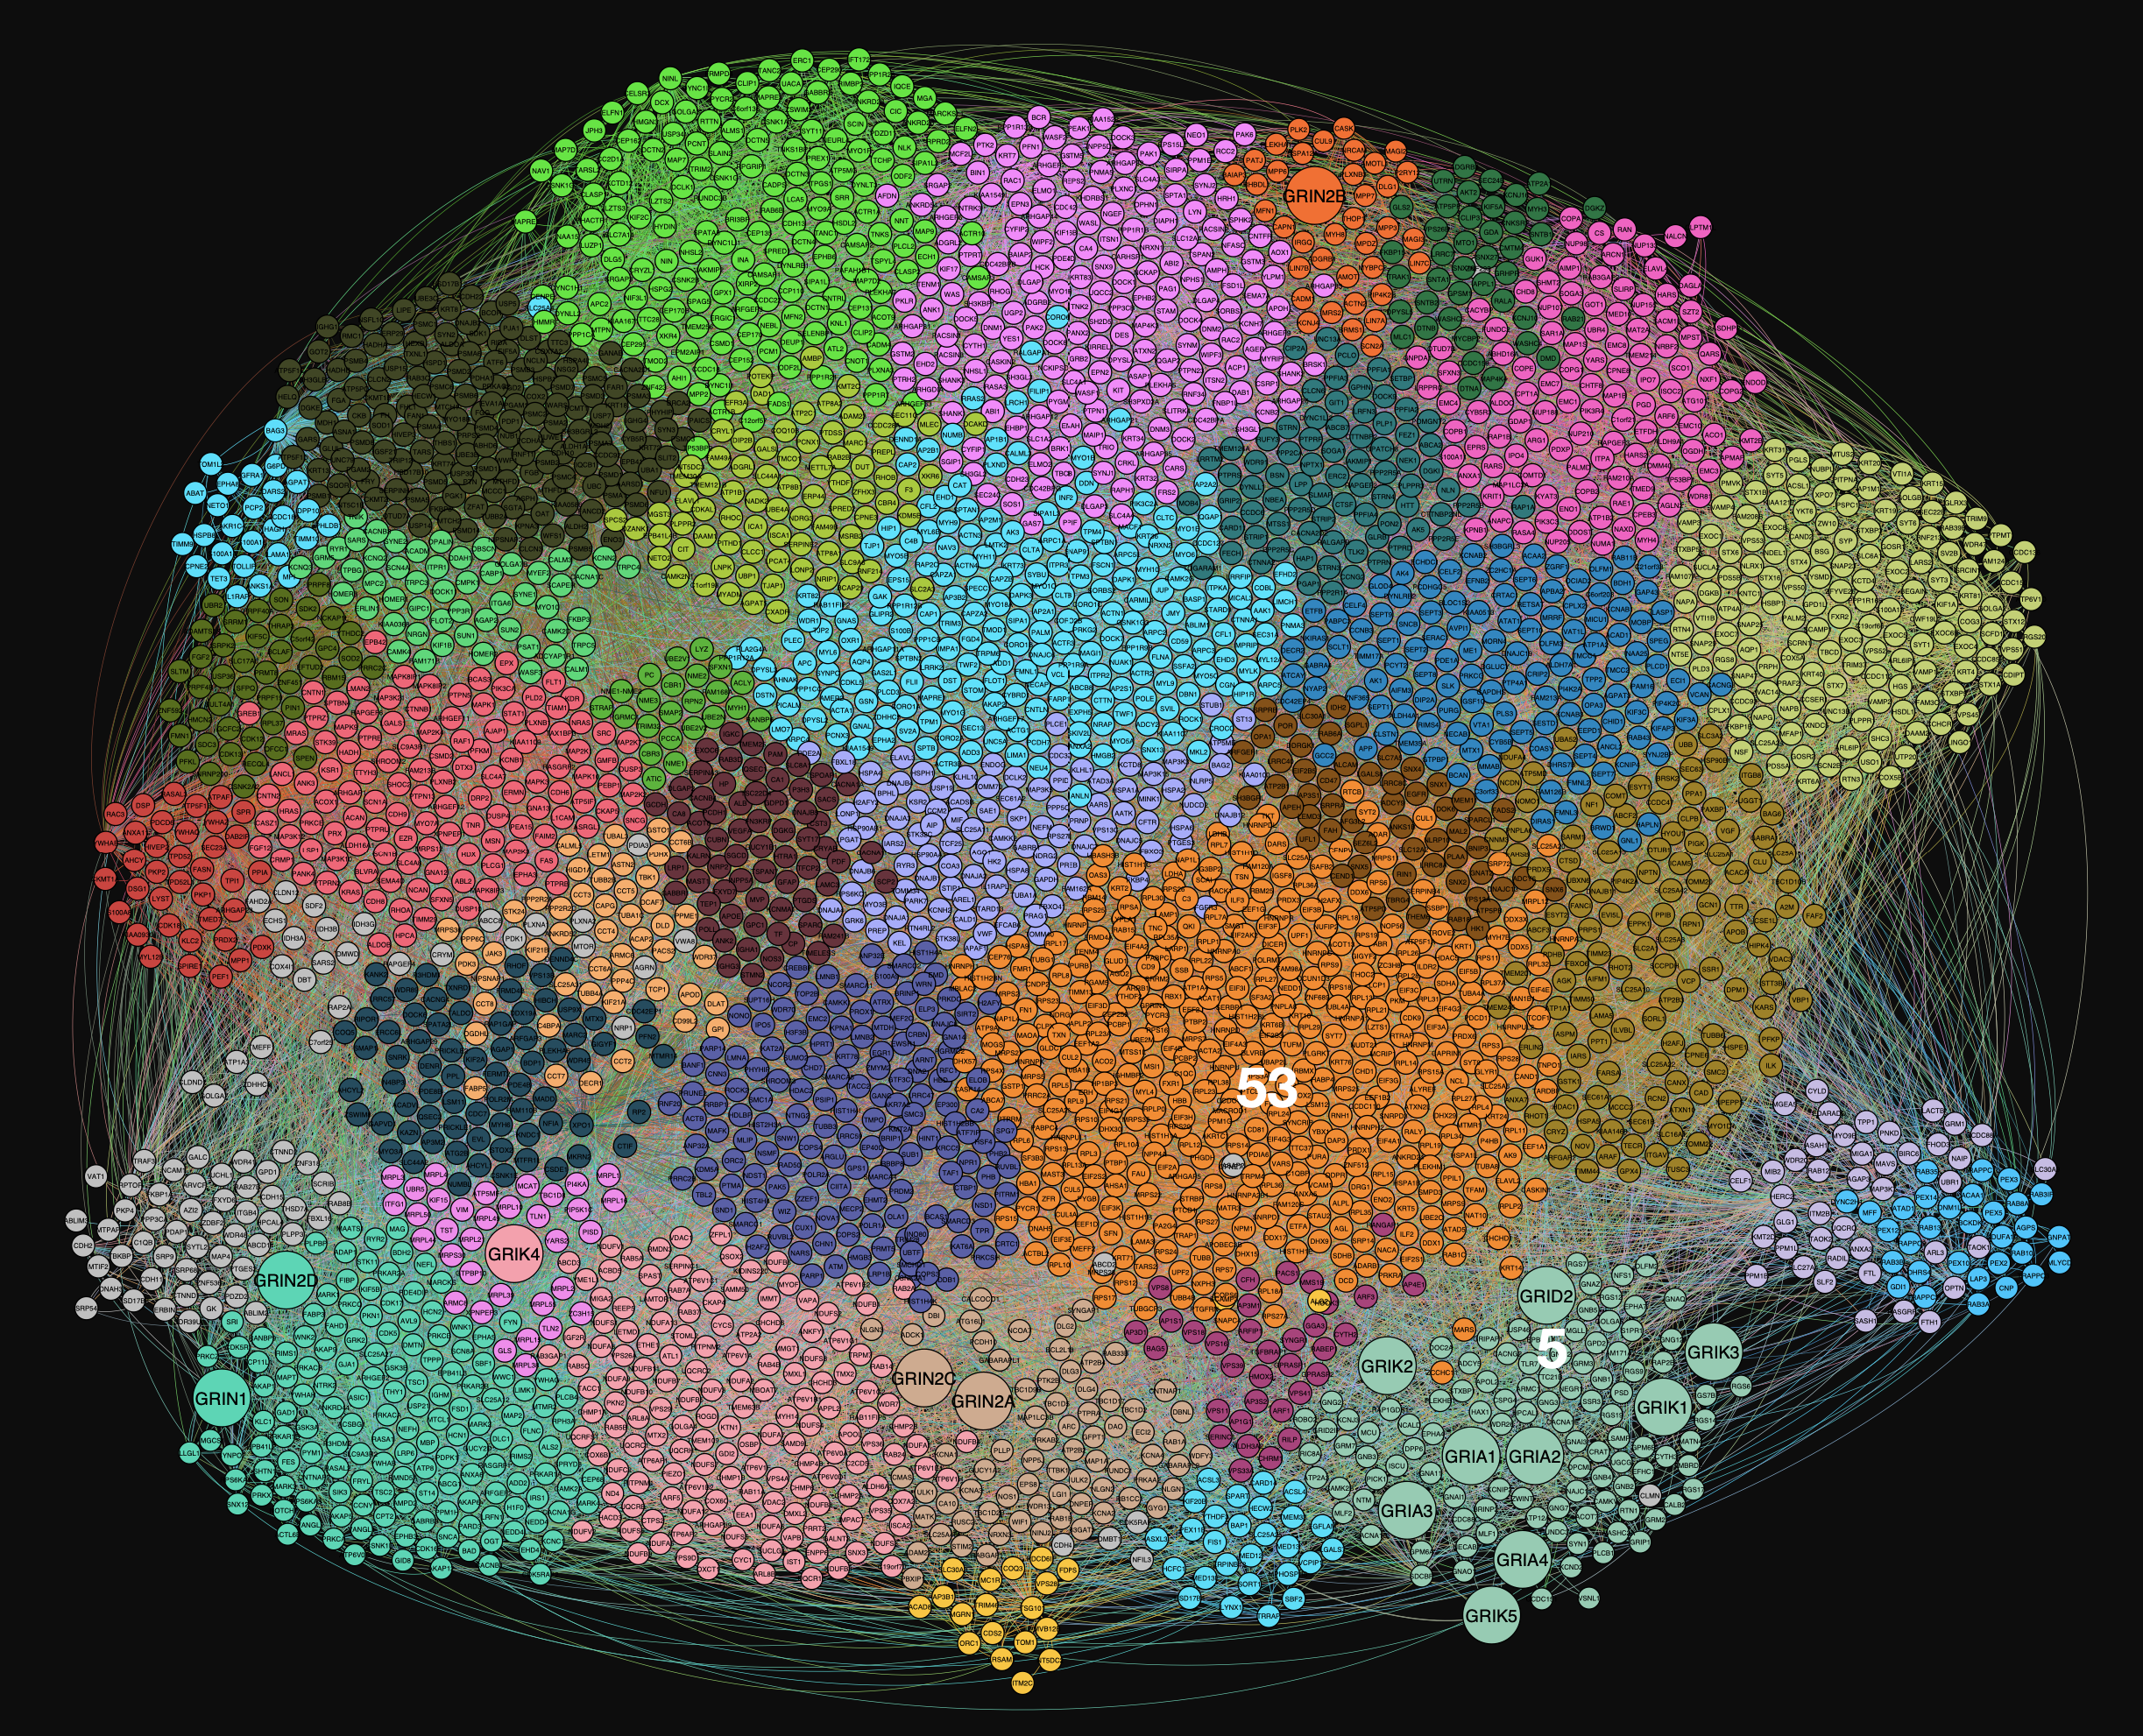
\includegraphics[width=0.9\textwidth]{images/chapter_community_detection/mac/psp.png}
    \caption{PSP visualised in Gephi. Group 5 and 53 labelled. Glutamate receptors are highlighted by using larger node size}
    \label{fig:communities_spectral}
\end{figure}


% latex table generated in R 3.6.3 by xtable 1.8-4 package
% Tue Apr  7 17:38:02 2020

\begin{figure}
    \centering
    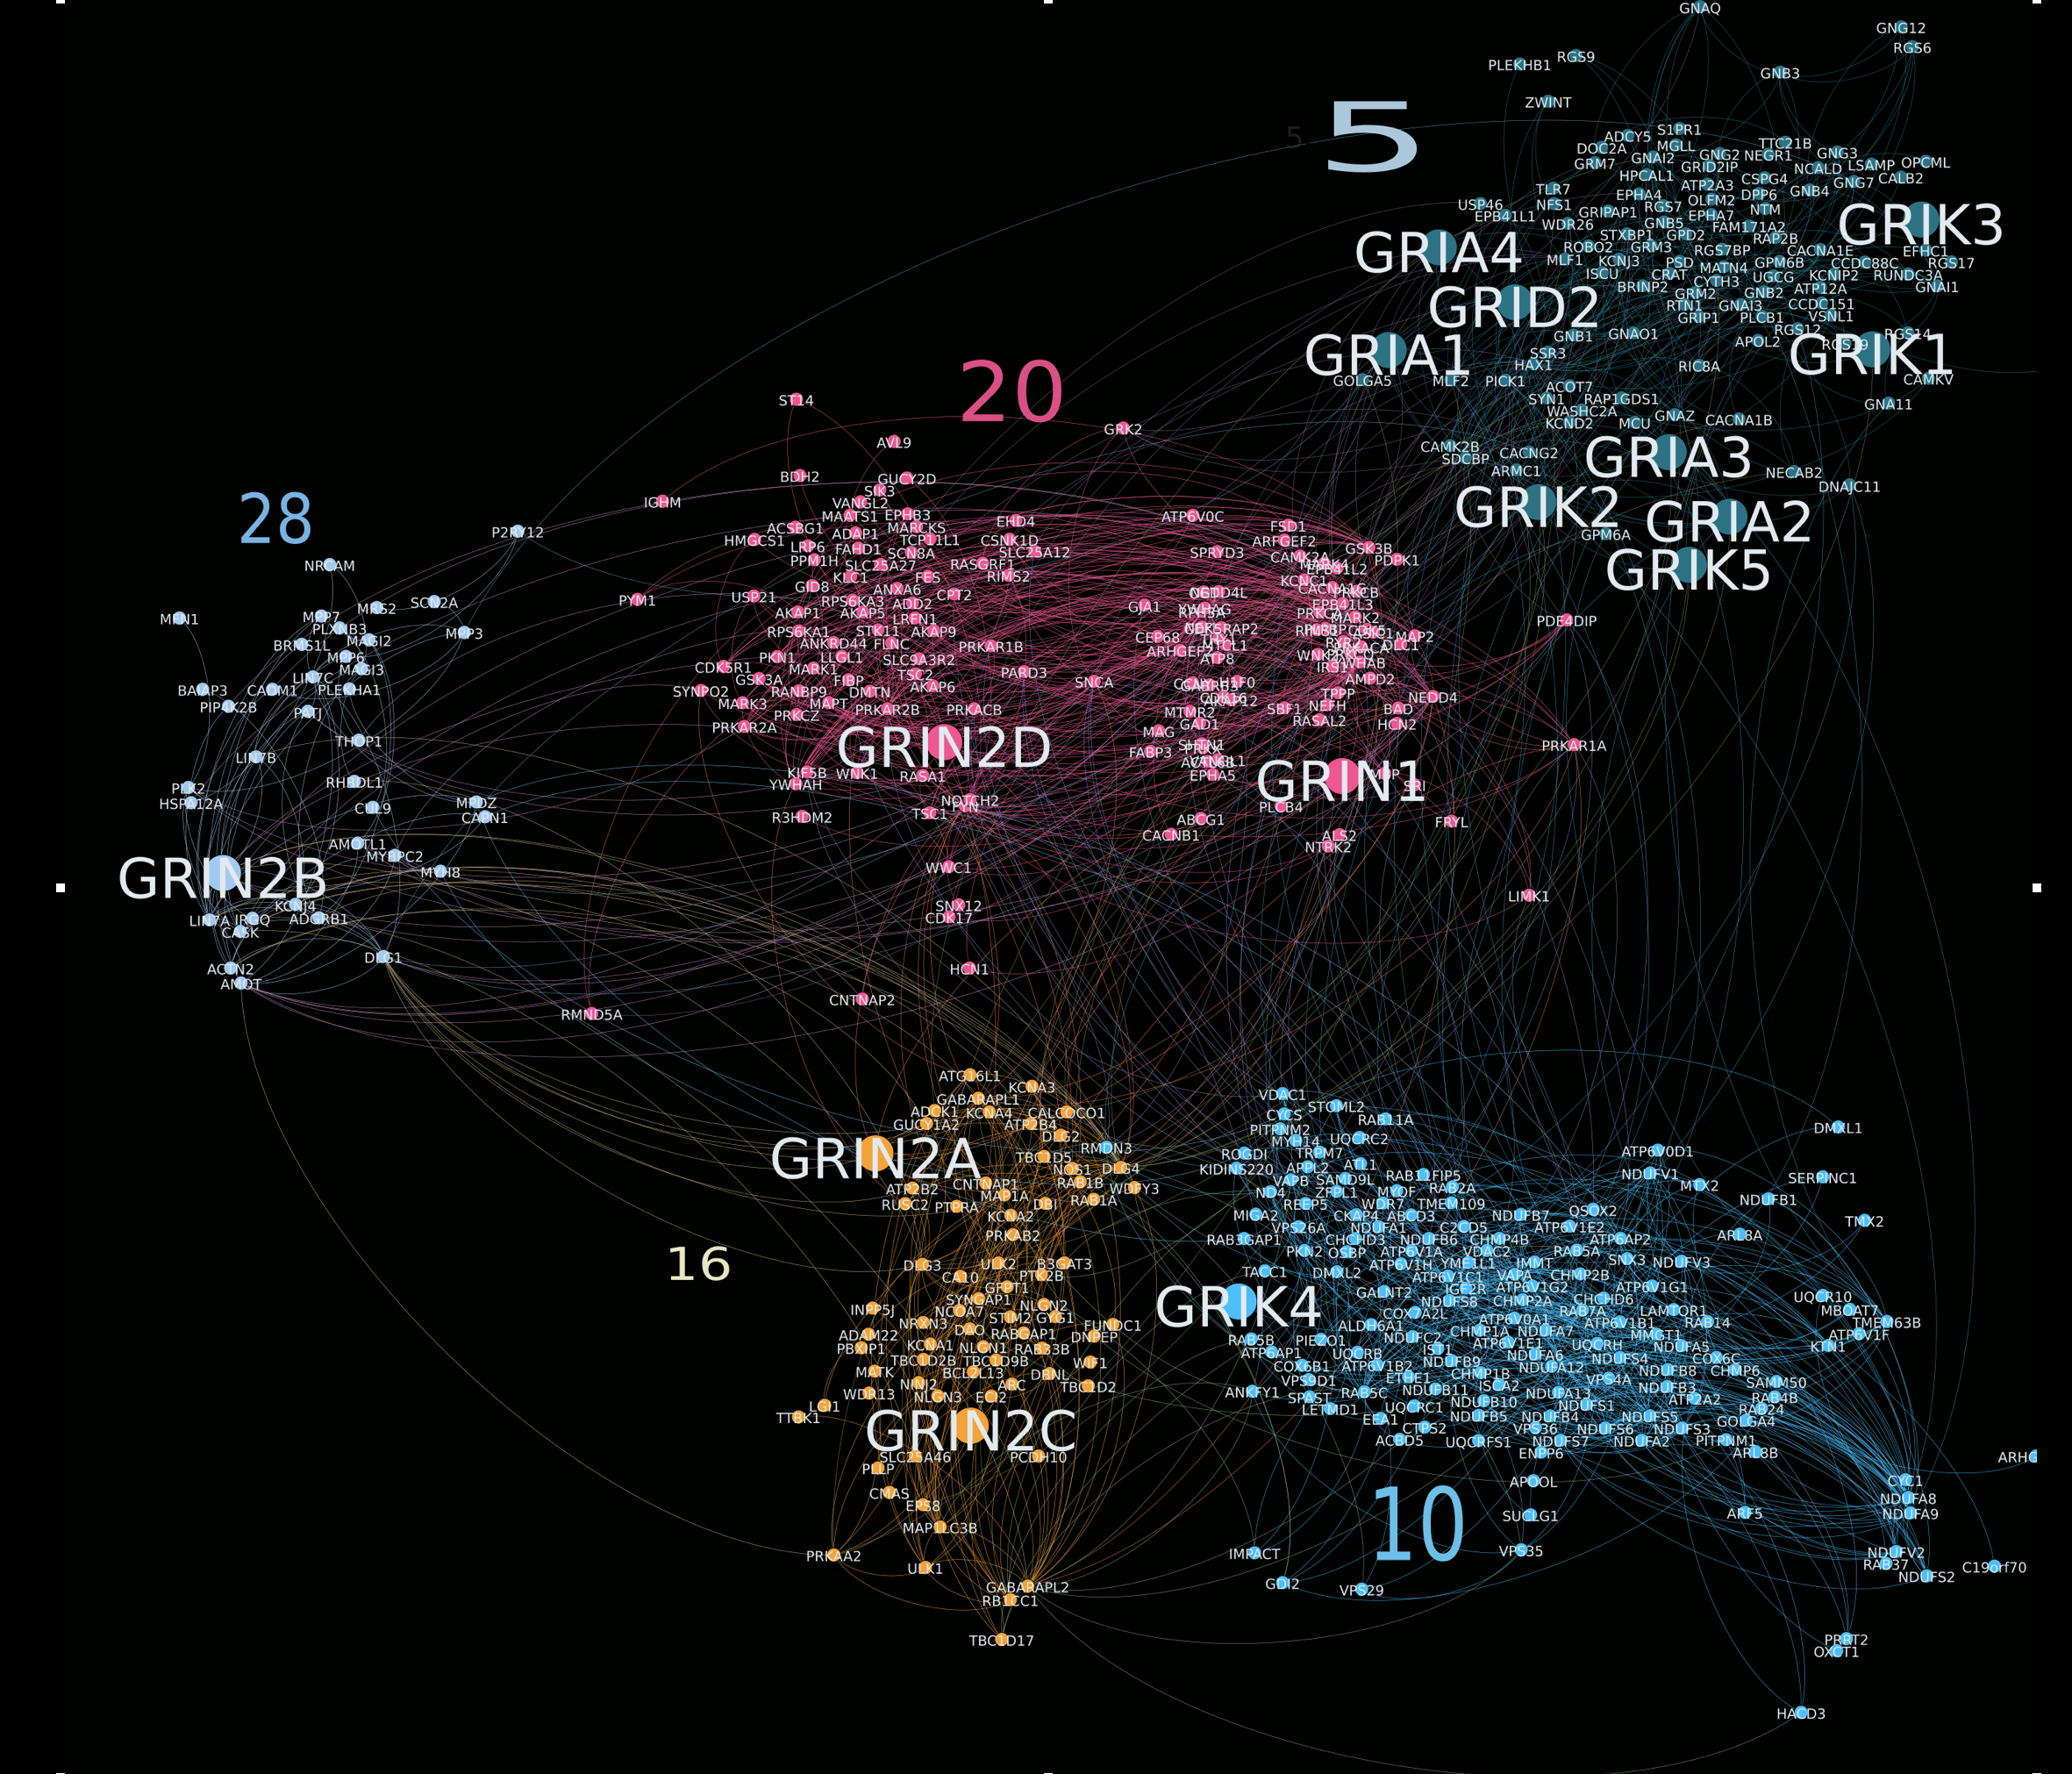
\includegraphics[width=0.9\textwidth]{images/chapter_community_detection/spectral_groups.png}
    \caption{Distribution of glutamate receptors across spectral groups and interconnections}
    \label{fig:communities_spectral}
\end{figure}




\begin{figure}
    \centering
    \includegraphics[width=\textwidth]{images/chapter_community_detection/gephi/show_groups_spectral1.png}
    \caption{Spectral groups}
    \label{fig:spectral groups}
\end{figure}

\subsubsection{Gene set enrichment results}

\paragraph{Educational attainment}
Four of 35 communities showed greater than nominally ($p<$0.05) significant enrichment using MAGMA\textsubscript{GSA} in the Education\textsubscript{Discovery} sample (community 5, $p$\textsubscript{MAGMA}=0.002, number of genes=106 ; community 53 $n$=405, $p$\textsubscript{MAGMA}=0.015 ; community 22 $n$=42, P\textsubscript{MAGMA}=0.035; community 47, P\textsubscript{MAGMA}= 0.035 n=47) (table~\ref{tab:MAGMA GSA Education  BE}). All communities other than 53 were among those ($n=7$) showing nominally significant enrichment using GSEA (5,11,20,22,24,33,47) and so communities 5 ($p$\textsubscript{GSEA}= 0.004), 22($p$\textsubscript{GSEA}= 0.014) and 47 ($p$\textsubscript{GSEA}= 0.017) were tested using the replication samples. $p$\textsubscript{GSEA} for community 53 was 0.29 (table~\ref{tab:Significant gene sets Educational Attaintment}). 

% latex table generated in R 3.6.3 by xtable 1.8-4 package
% Sun Apr  4 13:58:07 2021

\begin{table}[ht]
\centering
\setlength{\extrarowheight}{2pt}
\begin{tabular}{cllllllllll}
  \toprule
   &  \multicolumn{5}{c}{\textit{Discovery}} & \multicolumn{5}{c}{\textit{Replication}} \\
    \cmidrule{2-11}
Community & $n$ & $\beta$ & $\beta$ STD & SE & $p$ & $n$ & $\beta$ & $\beta$ STD & SE & $p$\\ 
  \midrule
1 & 161 & -0.03 & -0.00 & 0.07 & 0.639 & 162 & 0.05 & 0.01 & 0.07 & 0.207 \\ 
  2 & 153 & 0.10 & 0.01 & 0.08 & 0.093 & 153 & -0.07 & -0.01 & 0.07 & 0.867 \\ 
  3 & 39 & 0.22 & 0.01 & 0.16 & 0.082 & 39 & 0.09 & 0.00 & 0.14 & 0.260 \\ 
  4 & 29 & -0.17 & -0.01 & 0.18 & 0.821 & 30 & -0.36 & -0.01 & 0.15 & 0.991 \\ 
  \textbf{5} & 106 & 0.22 & 0.02 & 0.10 & \textbf{0.014} & 106 & 0.21 & 0.02 & 0.09 & \textbf{0.009} \\ 
  6 & 76 & -0.07 & -0.00 & 0.12 & 0.715 & 77 & 0.09 & 0.01 & 0.10 & 0.170 \\ 
  7 & 125 & 0.14 & 0.01 & 0.09 & 0.052 & 125 & -0.08 & -0.01 & 0.08 & 0.840 \\ 
  9 & 61 & -0.01 & -0.00 & 0.12 & 0.545 & 61 & 0.23 & 0.01 & 0.11 & 0.016 \\ 
  \textbf{10} & 146 & 0.19 & 0.02 & 0.08 & \textbf{0.008} & 146 & 0.02 & 0.00 & 0.07 & 0.375 \\ 
  11 & 55 & 0.14 & 0.01 & 0.13 & 0.145 & 55 & -0.11 & -0.01 & 0.11 & 0.848 \\ 
  12 & 32 & -0.01 & -0.00 & 0.16 & 0.522 & 32 & 0.18 & 0.01 & 0.15 & 0.113 \\ 
  16 & 68 & 0.00 & 0.00 & 0.12 & 0.494 & 68 & 0.21 & 0.01 & 0.10 & 0.022 \\ 
  17 & 144 & 0.02 & 0.00 & 0.08 & 0.417 & 144 & -0.00 & -0.00 & 0.07 & 0.506 \\ 
  19 & 20 & 0.21 & 0.01 & 0.18 & 0.124 & 20 & 0.10 & 0.00 & 0.15 & 0.262 \\ 
  20 & 144 & 0.13 & 0.01 & 0.09 & 0.070 & 144 & 0.13 & 0.01 & 0.07 & 0.039 \\ 
  \textbf{22} & 42 & 0.24 & 0.01 & 0.14 & \textbf{0.047} & 42 & -0.06 & -0.00 & 0.13 & 0.669 \\ 
  23 & 67 & -0.08 & -0.00 & 0.12 & 0.741 & 67 & -0.17 & -0.01 & 0.10 & 0.954 \\ 
  24 & 74 & 0.10 & 0.01 & 0.12 & 0.191 & 74 & 0.18 & 0.01 & 0.10 & 0.032 \\ 
  25 & 26 & 0.01 & 0.00 & 0.19 & 0.487 & 26 & -0.03 & -0.00 & 0.16 & 0.582 \\ 
  26 & 117 & 0.10 & 0.01 & 0.09 & 0.130 & 116 & 0.06 & 0.00 & 0.08 & 0.245 \\ 
  28 & 35 & -0.04 & -0.00 & 0.17 & 0.603 & 35 & 0.34 & 0.01 & 0.15 & 0.011 \\ 
  32 & 50 & -0.05 & -0.00 & 0.15 & 0.635 & 50 & 0.10 & 0.01 & 0.12 & 0.200 \\ 
  33 & 180 & 0.05 & 0.00 & 0.07 & 0.270 & 180 & 0.10 & 0.01 & 0.06 & 0.062 \\ 
  34 & 210 & 0.06 & 0.01 & 0.07 & 0.216 & 211 & -0.09 & -0.01 & 0.06 & 0.937 \\ 
  43 & 137 & 0.02 & 0.00 & 0.08 & 0.389 & 139 & -0.03 & -0.00 & 0.07 & 0.656 \\ 
  44 & 101 & 0.02 & 0.00 & 0.09 & 0.434 & 101 & -0.00 & -0.00 & 0.08 & 0.505 \\ 
  45 & 118 & 0.09 & 0.01 & 0.09 & 0.139 & 119 & 0.03 & 0.00 & 0.07 & 0.335 \\ 
  46 & 47 & 0.07 & 0.00 & 0.12 & 0.283 & 47 & 0.06 & 0.00 & 0.10 & 0.264 \\ 
  47 & 23 & 0.22 & 0.01 & 0.20 & 0.132 & 24 & -0.05 & -0.00 & 0.18 & 0.619 \\ 
  48 & 22 & 0.03 & 0.00 & 0.20 & 0.445 & 22 & -0.05 & -0.00 & 0.21 & 0.592 \\ 
  51 & 110 & -0.06 & -0.00 & 0.09 & 0.750 & 110 & 0.13 & 0.01 & 0.08 & 0.038 \\ 
  53 & 386 & 0.08 & 0.01 & 0.05 & 0.050 & 387 & 0.08 & 0.01 & 0.04 & 0.024 \\ 
  55 & 42 & 0.22 & 0.01 & 0.15 & 0.069 & 42 & 0.04 & 0.00 & 0.12 & 0.371 \\ 
  58 & 36 & -0.10 & -0.00 & 0.16 & 0.738 & 36 & -0.01 & -0.00 & 0.14 & 0.543 \\ 
  62 & 34 & -0.06 & -0.00 & 0.15 & 0.656 & 34 & -0.18 & -0.01 & 0.14 & 0.905 \\ 
   \bottomrule
\end{tabular}
\caption[MAGMA GSA Intelligence]{MAGMA GSA Intelligence  $\beta$ is the regression coefficient of the gene set. SE is the standard error of the regression coefficient. $\beta$ STD the semi-standardised regression coefficient, corresponding to the predicted
change in Z-value given a change of one standard deviation in the predictor gene set  gene covariate.  Note that the number of genes refers to the number of genes tested in MAGMA which may be less than the number of genes in the community as some genes may have no assigned SNPs.} 
\tiny\url{source('~/RProjects/chapter_community_detection/R/magma_gsa/intelligence_gsa_table.R')}\\
Redo 2021 \url{source('~/RProjects/chapter_community_detection/R/magma_gsa/rawread/intelligence_gsa_new_raw_table.R')}
\label{tab:MAGMA GSA Intelligence }
\end{table}



\begin{table}[ht]
\centering
\setlength{\extrarowheight}{2pt}
\begin{tabular}{cllllllllll}
  \toprule
   &  \multicolumn{5}{c}{\textit{Discovery}} & \multicolumn{5}{c}{\textit{Replication}} \\
    \cmidrule{2-11}
Community & $n$ & $\beta$ & $\beta$ STD & SE & $p$ & $n$ & $\beta$ & $\beta$ STD & SE & $p$\\ 
  \midrule
1 & 161 & 0.10 & 0.01 & 0.08 & 0.104 & 160 & 0.07 & 0.01 & 0.07 & 0.169 \\ 
  2 & 153 & 0.09 & 0.01 & 0.08 & 0.120 & 153 & 0.17 & 0.02 & 0.07 & 0.012 \\ 
  3 & 39 & -0.21 & -0.01 & 0.16 & 0.905 & 39 & -0.02 & -0.00 & 0.14 & 0.556 \\ 
  4 & 29 & -0.30 & -0.01 & 0.19 & 0.944 & 29 & -0.12 & -0.00 & 0.15 & 0.789 \\ 
  5 & 106 & 0.29 & 0.02 & 0.10 & \textbf{0.002} & 106 & 0.20 & 0.02 & 0.09 & \textbf{0.015} \\ 
  6 & 76 & 0.01 & 0.00 & 0.12 & 0.454 & 76 & 0.10 & 0.01 & 0.10 & 0.162 \\ 
  7 & 125 & 0.01 & 0.00 & 0.09 & 0.470 & 123 & -0.09 & -0.01 & 0.08 & 0.867 \\ 
  9 & 61 & 0.10 & 0.01 & 0.12 & 0.191 & 61 & 0.03 & 0.00 & 0.11 & 0.402 \\ 
  10 & 146 & 0.09 & 0.01 & 0.08 & 0.133 & 146 & 0.06 & 0.01 & 0.07 & 0.206 \\ 
  11 & 55 & -0.02 & -0.00 & 0.14 & 0.570 & 55 & -0.05 & -0.00 & 0.11 & 0.665 \\ 
  12 & 32 & 0.11 & 0.00 & 0.16 & 0.244 & 32 & 0.19 & 0.01 & 0.16 & 0.112 \\ 
  16 & 68 & -0.14 & -0.01 & 0.12 & 0.868 & 68 & 0.06 & 0.00 & 0.11 & 0.282 \\ 
  17 & 144 & -0.02 & -0.00 & 0.08 & 0.605 & 144 & -0.05 & -0.00 & 0.07 & 0.754 \\ 
  19 & 20 & 0.01 & 0.00 & 0.19 & 0.475 & 20 & 0.02 & 0.00 & 0.19 & 0.464 \\ 
  20 & 144 & 0.00 & 0.00 & 0.09 & 0.489 & 142 & 0.22 & 0.02 & 0.08 & 0.002 \\ 
  22 & 42 & 0.27 & 0.01 & 0.15 & 0.035 & 41 & 0.09 & 0.00 & 0.13 & 0.250 \\ 
  23 & 67 & -0.00 & -0.00 & 0.12 & 0.509 & 67 & 0.12 & 0.01 & 0.11 & 0.125 \\ 
  24 & 74 & 0.10 & 0.01 & 0.12 & 0.188 & 74 & 0.12 & 0.01 & 0.11 & 0.122 \\ 
  25 & 26 & -0.51 & -0.02 & 0.20 & 0.995 & 26 & 0.12 & 0.00 & 0.17 & 0.238 \\ 
  26 & 117 & 0.08 & 0.01 & 0.10 & 0.209 & 116 & -0.09 & -0.01 & 0.09 & 0.841 \\ 
  28 & 35 & -0.13 & -0.01 & 0.17 & 0.783 & 35 & 0.09 & 0.00 & 0.15 & 0.289 \\ 
  32 & 50 & 0.17 & 0.01 & 0.15 & 0.130 & 49 & -0.24 & -0.01 & 0.14 & 0.961 \\ 
  33 & 180 & 0.10 & 0.01 & 0.08 & 0.097 & 180 & 0.12 & 0.01 & 0.07 & 0.049 \\ 
  34 & 210 & 0.02 & 0.00 & 0.07 & 0.400 & 209 & -0.02 & -0.00 & 0.06 & 0.620 \\ 
  43 & 137 & -0.04 & -0.00 & 0.08 & 0.669 & 137 & 0.01 & 0.00 & 0.08 & 0.448 \\ 
  44 & 101 & -0.02 & -0.00 & 0.10 & 0.563 & 100 & -0.01 & -0.00 & 0.08 & 0.562 \\ 
  45 & 118 & 0.03 & 0.00 & 0.09 & 0.374 & 118 & 0.04 & 0.00 & 0.08 & 0.294 \\ 
  46 & 47 & 0.12 & 0.01 & 0.13 & 0.169 & 47 & 0.11 & 0.01 & 0.12 & 0.167 \\ 
  47 & 23 & 0.37 & 0.01 & 0.20 & 0.035 & 23 & -0.05 & -0.00 & 0.21 & 0.599 \\ 
  48 & 22 & 0.07 & 0.00 & 0.21 & 0.374 & 22 & 0.07 & 0.00 & 0.22 & 0.367 \\ 
  51 & 110 & 0.01 & 0.00 & 0.09 & 0.466 & 110 & -0.04 & -0.00 & 0.08 & 0.710 \\ 
  53 & 386 & 0.11 & 0.02 & 0.05 & 0.015 & 381 & 0.06 & 0.01 & 0.04 & 0.085 \\ 
  55 & 42 & 0.05 & 0.00 & 0.15 & 0.378 & 42 & -0.16 & -0.01 & 0.15 & 0.855 \\ 
  58 & 36 & -0.12 & -0.01 & 0.16 & 0.767 & 35 & -0.05 & -0.00 & 0.16 & 0.629 \\ 
  62 & 34 & -0.14 & -0.01 & 0.16 & 0.808 & 34 & -0.14 & -0.01 & 0.14 & 0.826 \\ 
   \bottomrule
\end{tabular}
\caption[MAGMA GSA Educational attainment]{MAGMA GSA Educational attainment  $\beta$ is the regression coefficient of the gene set. SE is the standard error of the regression coefficient. $\beta$ STD the the semi-standardized regression coefficient, corresponding to the predicted
change in Z-value given a change of one standard deviation in the predictor gene set / gene covariate. Note that the number of genes refers to the number of genes tested in MAGMA which may be less than the number of genes in the community as some genes may have no assigned SNPs. } 
    \tiny\url{source('~/RProjects/chapter_community_detection/R/magma_gsa/education_gsa_table.R')}
\label{tab:MAGMA GSA Education  BE}
\end{table}

 


\paragraph{Intelligence}In the Intelligence\textsubscript{Discovery} sample four gene sets showed nominally significant enrichment using MAGMA\textsubscript{GSA} (community 10, $p$\textsubscript{MAGMA}=0.008, $n$=146; community 5 $p$\textsubscript{MAGMA}=0.014,  $n$=106; community 22, $p$=0.046 $n$=42; cluster 53 $p$=0.050, $n$=386). However, only community 5  the Intelligence\textsubscript{Discovery} sample showed at least nominally significant enrichment on GSEA (table~\ref{tab:Significant gene sets GSEA Intelligence}) and MAGMA GSA ($p\textsubscript{MAGMA}<$0.05; table~\ref{tab:MAGMA GSA Intelligence }) and was analysed in the replication sample.

\paragraph{Replication}
 Community 5 was confirmed to have an enriched association with educational attainment in the Education\textsubscript{Replication} sample $p$\textsubscript{MAGMA}=0.01548, $p$\textsubscript{MAGMA} 0.045 Bonferroni ; Community 5 genes also were enriched in the Intelligence\textsubscript{Replication cohort} (p\textsubscript{MAGMA} = 0.0084 , table~\ref{tab:MAGMA GSA Intelligence } ; p\textsubscript{GSEA}=0.003,  table~\ref{tab:Significant gene sets GSEA Intelligence})




\begin{table}[ht!]
\centering
\setlength{\extrarowheight}{2pt}
\begin{tabular}{lllllll}
  \toprule
   &  \multicolumn{3}{c}{\textit{Discovery}} & \multicolumn{3}{c}{\textit{Replication}} \\
   \cmidrule{2-7}
Community & $n$ & ES & $p$ & $n$ & ES & $p$ \\ 
  \midrule
24 & 73 & 0.61 & 0.002 & 73 & 0.58 & 0.004 \\ 
  33 & 179 & 0.54 & 0.002 & 179 & 0.52 & 0.003 \\ 
  5 & 105 & 0.58 & 0.006 & 105 & 0.52 & 0.015 \\ 
  47 & 22 & 0.70 & 0.009 &  &  &  \\ 
  20 & 143 & 0.55 & 0.015 & 141 & 0.52 & 0.005 \\ 
  22 & 41 & 0.62 & 0.018 &  &  &  \\ 
  11 & 54 & 0.58 & 0.024 &  &  &  \\ 
  55 &  &  &  & 41 & 0.64 & 0.003 \\ 
  9 &  &  &  & 60 & 0.59 & 0.006 \\ 
  43 &  &  &  & 136 & 0.52 & 0.014 \\ 
   \bottomrule
\end{tabular}
\caption{Significant gene sets. GSEA Educational Attaintment. Discovery and replication cohorts.  ES = Enrichment score. n = number of genes in gene set, $p$= nominal p value} 
\tiny\url{source('~/RProjects/chapter_community_detection/R/gsea/format_sig_educational.R')}
\label{tab:Significant gene sets Educational Attaintment}
\end{table}

% latex table generated in R 3.6.3 by xtable 1.8-4 package
% Tue Mar 30 17:09:20 2021
\begin{table}[ht!]
\centering
\setlength{\extrarowheight}{2pt}
\begin{tabular}{lllllll}
  \toprule
   &  \multicolumn{3}{c}{\textit{Discovery}} & \multicolumn{3}{c}{\textit{Replication}} \\
   \cmidrule{2-7}
Community & $n$ & ES & $p$ & $n$ & ES & $p$ \\ 
  \midrule
5 & 105 & 0.60 & 0.001 & 105 & 0.54 & 0.003 \\ 
  53 & 385 & 0.51 & 0.004 &  &  &  \\ 
  43 & 136 & 0.54 & 0.013 &  &  &  \\ 
  34 & 209 & 0.51 & 0.023 &  &  &  \\ 
  3 & 38 & 0.60 & 0.038 &  &  &  \\ 
  20 &  &  &  & 143 & 0.51 & 0.009 \\ 
  33 &  &  &  & 179 & 0.48 & 0.021 \\ 
  26 &  &  &  & 115 & 0.50 & 0.033 \\ 
   \bottomrule
\end{tabular}
\caption{Significant gene sets GSEA Intelligence Discovery and Replication samples.  ES = Enrichment score. $n$ = number of genes in gene set, $p$= nominal p value}
\tiny\url{source('~/RProjects/chapter_community_detection/R/gsea/format_sig_intelligence.R')}
\label{tab:Significant gene sets GSEA Intelligence}
\end{table}

The analysis was repeated using gene scoring and the pathway enrichment function in Pascal \cite{lamparter2016fast}. The results from the Intelligence\textsubscript{Discovery} and Intelligence\textsubscript{Replication} samples are shown in table~\ref{tab:Intelligence PASCAL}. Community Group 5 showed significant enrichment in all four cohorts using Pascal’s gene scoring and GSA analysis methods Education\textsubscript{Discovery} p=0.00007, Intelligence Discovery p=0.0001; Education Replication p=0.0003, Intelligence Replication p=0.0001; alpha Bonferroni=0.0015 table~\ref{tab:Intelligence PASCAL} and table~\ref{tab:Pascal Education ordered by chi2P}. The chi squared is reported following the authors `extreme case one gene might reach scores so high that it precludes detection of pathways not containing that gene when the empirical sampling strategy is used'\cite{lamparter2016fast}. Community five was the most enriched set in all samples tested in MAGMA. 

% latex table generated in R 3.6.3 by xtable 1.8-4 package
% Sun Apr  4 14:43:19 2021
\begin{table}[ht]
\centering
\setlength{\extrarowheight}{2pt}
\begin{tabular}{llllll}
  \toprule
   &  \multicolumn{2}{c}{\textit{Discovery}} & \multicolumn{2}{c}{\textit{Replication}} \\
   \cmidrule{2-5}
 Community & $\chi^2$ $p$ value  & emp $p$ value  & $\chi^2$ $p$ value   & emp $p$ value   \\ 
  \midrule
5 & 0.00005 & 0.00011 & 0.00005 & 0.00012 \\ 
  10 & 0.00118 & 0.00842 & 0.00215 & 0.00238 \\ 
  53 & 0.00551 & 0.00674 & 0.05289 & 0.04662 \\ 
  7 & 0.01457 & 0.03852 & 0.23362 & 0.17917 \\ 
  33 & 0.02126 & 0.06174 & 0.03314 & 0.03936 \\ 
  26 & 0.02152 & 0.03371 & 0.09655 & 0.12936 \\ 
  20 & 0.02629 & 0.05821 & 0.00142 & 0.00239 \\ 
  34 & 0.03021 & 0.07349 & 0.48926 & 0.45609 \\ 
  28 & 0.06082 & 0.06805 & 0.18416 & 0.23682 \\ 
  43 & 0.06633 & 0.03141 & 0.37601 & 0.41863 \\ 
  55 & 0.08403 & 0.13622 & 0.44314 & 0.47030 \\ 
  22 & 0.09465 & 0.07006 & 0.32361 & 0.26264 \\ 
  3 & 0.09514 & 0.07290 & 0.13478 & 0.11655 \\ 
  19 & 0.09847 & 0.05388 & 0.88967 & 0.86107 \\ 
  58 & 0.12710 & 0.10808 & 0.26938 & 0.19509 \\ 
  2 & 0.13497 & 0.16725 & 0.76900 & 0.73094 \\ 
  45 & 0.13872 & 0.15079 & 0.43880 & 0.38630 \\ 
  12 & 0.14885 & 0.21203 & 0.13265 & 0.17448 \\ 
  11 & 0.15258 & 0.13086 & 0.90882 & 0.89701 \\ 
  24 & 0.17389 & 0.16971 & 0.04770 & 0.06090 \\ 
  46 & 0.18991 & 0.18483 & 0.20068 & 0.22571 \\ 
  47 & 0.26565 & 0.24708 & 0.34319 & 0.29384 \\ 
  1 & 0.29315 & 0.32094 & 0.21352 & 0.24257 \\ 
  9 & 0.31205 & 0.38279 & 0.07316 & 0.09553 \\ 
  23 & 0.33463 & 0.39840 & 0.64103 & 0.66756 \\ 
  32 & 0.33661 & 0.41270 & 0.17894 & 0.21654 \\ 
  44 & 0.36507 & 0.39839 & 0.57021 & 0.53741 \\ 
  17 & 0.37087 & 0.31369 & 0.35273 & 0.31447 \\ 
  25 & 0.44107 & 0.44977 & 0.44278 & 0.45825 \\ 
  51 & 0.45466 & 0.56525 & 0.07424 & 0.08153 \\ 
  62 & 0.65120 & 0.63921 & 0.47485 & 0.49011 \\ 
  48 & 0.65913 & 0.65999 & 0.82988 & 0.82570 \\ 
  16 & 0.73722 & 0.70116 & 0.08981 & 0.11902 \\ 
  6 & 0.76799 & 0.74957 & 0.39325 & 0.31039 \\ 
  4 & 0.80237 & 0.78159 & 0.96353 & 0.96408 \\ 
   \bottomrule
\end{tabular}
\caption[GSA PASCAL Intelligence]{Intelligence samples PASCAL GSA Discovery and Replication samples ordered by $\chi^2$ $p$ value. emp = empirical p value method.}
\label{tab:Intelligence PASCAL}
\end{table}


% latex table generated in R 3.6.3 by xtable 1.8-4 package
% Sun Apr  4 14:55:16 2021
\begin{table}[ht]
\centering
\setlength{\extrarowheight}{2pt}
\begin{tabular}{llllll}
  \toprule
   &  \multicolumn{2}{c}{\textit{Discovery}} & \multicolumn{2}{c}{\textit{Replication}} \\
   \cmidrule{2-5}
  Community & $\chi^2$ $p$ value  & emp $p$ value  & $\chi^2$ $p$ value   & emp $p$ value   \\ 
  \midrule
5 & 0.00006 & 0.00007 & 0.00101 & 0.00026 \\ 
  20 & 0.00009 & 0.00064 & 0.00019 & 0.00214 \\ 
  2 & 0.00010 & 0.00197 & 0.02859 & 0.05484 \\ 
  33 & 0.00033 & 0.00351 & 0.00774 & 0.03373 \\ 
  47 & 0.01040 & 0.03107 & 0.29248 & 0.30947 \\ 
  24 & 0.01135 & 0.00904 & 0.00121 & 0.00124 \\ 
  53 & 0.01668 & 0.03576 & 0.44041 & 0.57615 \\ 
  22 & 0.01690 & 0.04507 & 0.17748 & 0.17328 \\ 
  1 & 0.04775 & 0.04565 & 0.19103 & 0.20056 \\ 
  11 & 0.04848 & 0.02619 & 0.24541 & 0.10527 \\ 
  10 & 0.04947 & 0.12340 & 0.14220 & 0.12294 \\ 
  34 & 0.06379 & 0.09816 & 0.02931 & 0.08681 \\ 
  32 & 0.07427 & 0.14669 & 0.88655 & 0.88639 \\ 
  26 & 0.12693 & 0.11476 & 0.29690 & 0.21301 \\ 
  51 & 0.12879 & 0.19808 & 0.06750 & 0.10246 \\ 
  44 & 0.13406 & 0.21763 & 0.12548 & 0.22032 \\ 
  46 & 0.16189 & 0.17636 & 0.37360 & 0.40041 \\ 
  7 & 0.20011 & 0.23541 & 0.44014 & 0.47564 \\ 
  4 & 0.21800 & 0.27362 & 0.94031 & 0.93664 \\ 
  12 & 0.22076 & 0.24324 & 0.12664 & 0.19635 \\ 
  45 & 0.22085 & 0.33226 & 0.34137 & 0.41257 \\ 
  55 & 0.23156 & 0.31491 & 0.04923 & 0.05854 \\ 
  9 & 0.23518 & 0.32986 & 0.03420 & 0.07557 \\ 
  19 & 0.29122 & 0.33875 & 0.37543 & 0.39652 \\ 
  3 & 0.31886 & 0.27426 & 0.34172 & 0.35703 \\ 
  28 & 0.33989 & 0.36836 & 0.19262 & 0.26534 \\ 
  23 & 0.39185 & 0.47784 & 0.58355 & 0.61850 \\ 
  6 & 0.42214 & 0.46701 & 0.70931 & 0.70462 \\ 
  17 & 0.42623 & 0.47928 & 0.60287 & 0.57664 \\ 
  16 & 0.43234 & 0.51029 & 0.31117 & 0.42090 \\ 
  43 & 0.47397 & 0.47877 & 0.00273 & 0.00416 \\ 
  48 & 0.49223 & 0.46679 & 0.55516 & 0.56118 \\ 
  58 & 0.71790 & 0.74793 & 0.62110 & 0.65671 \\ 
  62 & 0.96246 & 0.96134 & 0.19788 & 0.25513 \\ 
  25 & 0.96330 & 0.96085 & 0.64162 & 0.65989 \\ 
   \bottomrule
\end{tabular}
\caption[GSA PASCAL Educational attainment sample]{Educational attainment samples PASCAL GSA Discovery and Replication samples ordered by $\chi^2$ $p$ value. emp = empirical p value method.} 
\label{tab:Pascal Education ordered by chi2P}
\end{table}
\clearpage



\subsection{Gene ontology analysis}
\label{sec: spectral group 5 analysis}
Community 5 is significantly enriched for terms related to glutamate receptor activity and the heterotrimeric g protein complex, including the G protein coupled serotonin receptor. Community 5 has a significant proportion of these terms whether one compares against the rest of the genome or relative to other synaptic groups. 21 of the 27 genes annotated by the Gene Ontology Consortium as
glutamate receptor activity (GO:0008066 MF) are found in the PSP. Of these, 12 are found in group 5 (57.1\%). 
23 of the 37 genes encoding proteins annotated heterotrimeric g protein (GO:0005834) are found in the PSP. Of these, 16 are found in group 5 (69.5\% of PSP GO:0005834). 

ToppGene and PANTHER over-representation test was carried out for each of the GO clades, Biological Process, Molecular Function, Cellular Component with the gene set compared with the 3.457 PSP genes. The ToppGene results ordered by FDR are shown for Molecular Function (table~\ref{tab:Group 5 GO: Molecular Function 79 significant terms}), Biological Process (table~\ref{tab:Group 5 GO: Biological Process 84 significant terms} and Cellular Component~\ref{tab:Group 5 GO: Cellular Component 78 significant terms}).

The biological process (BP) with the lowest FDR p value was G protein coupled receptor signalling activity, GO:0007186 $n$=38, $n$ PSP=189, FDR $q$ $2.36 \times 10^{-18}$. The same term was top in PANTHER although the absolute enrichment level was different (GO:0007186: FDR $q$=$2.16\times10{-8}$, fold enrichment 4.23). The second lowest was  glutamate receptor signalling pathway  GO:0007215 $n$=17, $n$ PSP= 43 ,FDR $3.46 \times 10^{-12}$ (PANTHER, also second term GO 0007215: FDR $q$ 7.23 x 10-07, fold change 12.62). These two terms were used for subgroup analysis (section~\ref{sec:subgroup analysis}). 

Glutamate receptor activity GO:0008066 was also the most over represented molecular function term using both enrichment methods: ToppGene $n=$12,  $n PSP=21$,  $6.96 \times 10^{-11}$ (PANTHER FDR 7.58 x 10-07, fold change 16). The most enriched cellular component was GTPase complex GO:1905360: $n$=16 , $n$ PSP=22, FDR $q$=$6.40 \times 10^{-18}$ (PANTHER FDR $8.75\times10^{-8}$, fold change 18.23, also first). This was followed by heterotrimeric G-protein complex:GO:0005834 $n$= 16 , $n$ PSP= 22, FDR $q$=$6.40 \times 10^{-18}$ (PANTHER FDR $q=1.75\times 10^{-7}$, fold change 18.23).


% latex table generated in R 3.6.3 by xtable 1.8-4 package
% Sun Apr  4 15:28:14 2021
% latex table generated in R 3.6.3 by xtable 1.8-4 package
% Sun Apr  4 15:35:07 2021
\begin{table}[ht]
\centering
\setlength{\extrarowheight}{2pt}
\begin{adjustbox}{width=\textwidth}
\begin{tabular}{llllll}
  \toprule
ID & Name & $n$ & $n$ PSP & $p$ & $q$ FDR B.H \\ 
  \midrule
GO:0008066 & glutamate receptor activity & 12 & 21 & $1.86 \times 10^{-13}$ & $6.96 \times 10^{-11}$ \\ 
  GO:0016595 & glutamate binding & 12 & 23 & $8.11 \times 10^{-13}$ & $1.52 \times 10^{-10}$ \\ 
  GO:0004970 & ionotropic glutamate receptor activity & 9 & 16 & $2.89 \times 10^{-10}$ & $3.60 \times 10^{-8}$ \\ 
  GO:0016597 & amino acid binding & 12 & 40 & $2.10 \times 10^{-9}$ & $1.96 \times 10^{-7}$ \\ 
  GO:1904315 & transmitter-gated ion channel activity  & 9 & 20 & $3.80 \times 10^{-9}$ & $2.84 \times 10^{-7}$ \\ 
  GO:0005230 & extracellular ligand-gated ion channel  & 9 & 21 & $6.47 \times 10^{-9}$ & $3.00 \times 10^{-7}$ \\ 
  GO:0022835 & transmitter-gated channel activity & 9 & 21 & $6.47 \times 10^{-9}$ & $3.00 \times 10^{-7}$ \\ 
  GO:0022824 & transmitter-gated ion channel activity & 9 & 21 & $6.47 \times 10^{-9}$ & $3.00 \times 10^{-7}$ \\ 
  GO:0031821 & G protein-coupled serotonin receptor bin & 6 & 7 & $7.23 \times 10^{-9}$ & $3.00 \times 10^{-7}$ \\ 
  GO:0099529 & neurotransmitter receptor activity invol & 9 & 22 & $1.06 \times 10^{-8}$ & $3.98 \times 10^{-7}$ \\ 
   \bottomrule
\end{tabular}
\end{adjustbox}
\caption[Community 5 Gene Ontology Analysis Molecular Function]{Community 5 GO: Molecular Function 79 significant terms} 
\tiny\url{source('~/RProjects/chapter_community_detection/R/group_enrichment/read_toppgene5/enrichMF.R')}
\label{tab:Group 5 GO: Molecular Function 79 significant terms}
\end{table}

% latex table generated in R 3.6.3 by xtable 1.8-4 package
% Sun Apr  4 15:49:05 2021
\begin{table}[ht]
\centering
\setlength{\extrarowheight}{2pt}
\begin{adjustbox}{width=\textwidth}
\begin{tabular}{llllll}
  \toprule
ID & Name &$n$ &$n$ PSP& $p$ & $q$ FDR B.H \\ 
  \midrule
GO:0007186 & G protein-coupled receptor signaling pathway & 38 & 189 & $9.89 \times 10^{-22}$ & $2.36 \times 10^{-18}$ \\ 
  GO:0007215 & glutamate receptor signaling pathway & 17 & 43 & $2.89 \times 10^{-15}$ & $3.46 \times 10^{-12}$ \\ 
  GO:0051339 & regulation of lyase activity & 18 & 66 & $7.30 \times 10^{-13}$ & $5.52 \times 10^{-10}$ \\ 
  GO:0098916 & anterograde trans-synaptic signaling & 42 & 414 & $1.16 \times 10^{-12}$ & $5.52 \times 10^{-10}$ \\ 
  GO:0007268 & chemical synaptic transmission & 42 & 414 & $1.16 \times 10^{-12}$ & $5.52 \times 10^{-10}$ \\ 
  GO:0099537 & trans-synaptic signaling & 42 & 420 & $1.91 \times 10^{-12}$ & $7.60 \times 10^{-10}$ \\ 
  GO:0007188 & adenylate cyclase-modulating G protein-c & 16 & 54 & $3.76 \times 10^{-12}$ & $1.09 \times 10^{-9}$ \\ 
  GO:0099536 & synaptic signaling & 42 & 429 & $3.98 \times 10^{-12}$ & $1.09 \times 10^{-9}$ \\ 
  GO:0045761 & regulation of adenylate cyclase activity & 17 & 63 & $4.09 \times 10^{-12}$ & $1.09 \times 10^{-9}$ \\ 
  GO:0031279 & regulation of cyclase activity & 17 & 65 & $7.15 \times 10^{-12}$ & $1.71 \times 10^{-9}$ \\ 
   \bottomrule
\end{tabular}
\end{adjustbox}
\caption[Community 5 Gene Ontology analysis Biological Process]{Community 5 GO: Biological Process 84 significant terms} 
\tiny\url{source('~/RProjects/chapter_community_detection/R/group_enrichment/read_toppgene5/enrichMF.R')}
\label{tab:Group 5 GO: Biological Process 84 significant terms}
\end{table}



% latex table generated in R 3.6.3 by xtable 1.8-4 package
% Sun Apr  4 15:57:37 2021
\begin{table}[ht]
\centering
\setlength{\extrarowheight}{2pt}
\begin{adjustbox}{width=\textwidth}
\begin{tabular}{llllll}
  \toprule
ID & Name &$n$ &$n$ PSP& $p$ & $q$ FDR B.H \\ 
  \midrule
GO:1905360 & GTPase complex & 16 & 22 & $3.44 \times 10^{-20}$ & $6.40 \times 10^{-18}$ \\ 
  GO:0005834 & heterotrimeric G-protein complex & 16 & 22 & $3.44 \times 10^{-20}$ & $6.40 \times 10^{-18}$ \\ 
  GO:0098797 & plasma membrane protein complex & 35 & 215 & $1.01 \times 10^{-16}$ & $1.25 \times 10^{-14}$ \\ 
  GO:0031234 & extrinsic component of cytoplasmic side  & 17 & 59 & $1.37 \times 10^{-12}$ & $1.28 \times 10^{-10}$ \\ 
  GO:0030425 & dendrite & 41 & 435 & $3.60 \times 10^{-11}$ & $2.23 \times 10^{-9}$ \\ 
  GO:0097447 & dendritic tree & 41 & 435 & $3.60 \times 10^{-11}$ & $2.23 \times 10^{-9}$ \\ 
  GO:0097060 & synaptic membrane & 29 & 243 & $2.53 \times 10^{-10}$ & $1.34 \times 10^{-8}$ \\ 
  GO:0019898 & extrinsic component of membrane & 24 & 174 & $6.13 \times 10^{-10}$ & $2.85 \times 10^{-8}$ \\ 
  GO:0036477 & somatodendritic compartment & 44 & 560 & $2.41 \times 10^{-9}$ & $9.85 \times 10^{-8}$ \\ 
  GO:0045211 & postsynaptic membrane & 22 & 157 & $2.65 \times 10^{-9}$ & $9.85 \times 10^{-8}$ \\ 
   \bottomrule
\end{tabular}
\end{adjustbox}
\caption{Group 5 GO: Cellular Component 78 significant terms} 
\tiny\url{source('~/RProjects/chapter_community_detection/R/group_enrichment/read_toppgene5/enrichCC.R')}
\label{tab:Group 5 GO: Cellular Component 78 significant terms}
\end{table}

    
\subsection{Murine and Disease Phenotypes in Community 5}
The genes within group 5 have a strongly-enriched association with murine phenotypes related to synaptic transmission (See table~\ref{tab:Group 5 Mouse Phenotype 28 significant terms} for enrichment with PSP background). 

The fifth term is  abnormal long term potentiation ( MP:0002207) 15 of 117 terms in PSP (12.8\% of terms 3.79 fold change compared with PSP) FDR q=$2.46 \times 10^{-3}$. Other terms are related to abnormal emotion, anxiety hyperactivity and fear related behaviour showing an effect from genes on both LTP and complex behaviour(see \cite{grant2018synaptomic},\cite{grant2019synapse}).







% latex table generated in R 3.6.3 by xtable 1.8-4 package
% Sun Apr  4 15:59:15 2021
\begin{table}[ht]
\centering
\setlength{\extrarowheight}{2pt}
\begin{adjustbox}{width=\textwidth}
\begin{tabular}{llllll}
  \toprule
ID & Name &$n$ &$n$ PSP& $p$ & $q$ FDR B.H \\ 
  \midrule
MP:0001970 & abnormal pain threshold & 12 & 64 & $1.48 \times 10^{-6}$ & $2.28 \times 10^{-3}$ \\ 
  MP:0020870 & decreased thigmotaxis & 9 & 40 & $6.96 \times 10^{-6}$ & $2.46 \times 10^{-3}$ \\ 
  MP:0002572 & abnormal emotion/affect behaviour & 30 & 377 & $7.30 \times 10^{-6}$ & $2.46 \times 10^{-3}$ \\ 
  MP:0001362 & abnormal anxiety-related response & 20 & 194 & $8.67 \times 10^{-6}$ & $2.46 \times 10^{-3}$ \\ 
  MP:0002207 & abnormal long term potentiation & 15 & 117 & $1.00 \times 10^{-5}$ & $2.46 \times 10^{-3}$ \\ 
  MP:0001399 & hyperactivity & 24 & 268 & $1.11 \times 10^{-5}$ & $2.46 \times 10^{-3}$ \\ 
  MP:0002065 & abnormal fear/anxiety-related behaviour & 22 & 232 & $1.12 \times 10^{-5}$ & $2.46 \times 10^{-3}$ \\ 
  MP:0003635 & abnormal synaptic transmission & 30 & 391 & $1.56 \times 10^{-5}$ & $2.99 \times 10^{-3}$ \\ 
  MP:0001968 & abnormal touch/ nociception & 12 & 82 & $2.20 \times 10^{-5}$ & $3.75 \times 10^{-3}$ \\ 
  MP:0009745 & abnormal behavioural response to xenobiot & 14 & 113 & $3.06 \times 10^{-5}$ & $4.70 \times 10^{-3}$ \\ 
   \bottomrule
\end{tabular}
\end{adjustbox}
\caption{Group 5 Mouse Phenotype 28 significant terms}
\tiny\url{source('~/RProjects/chapter_community_detection/R/group_enrichment/read_toppgene5/enrich_murine.R')}
\label{tab:Group 5 Mouse Phenotype 28 significant terms}
\end{table}


Community 5 has an enriched association with genes that have been reported to be implicated in the aetiology of common neuropsychiatric disorders. Using ToppGene to perform enrichment using terms in DisGeNet and the PSP as background the most enriched disorder is schizophrenia (C0036341 $n$=29, $n$ PSP=291 q=$2.28 \times 10^{-3}$. This is approximately 10\% of the terms annotated in the PSP. Depressive disorder also shows an enriched association (table~\ref{tab:Group 5 Disease 24 significant terms}).  




% latex table generated in R 3.6.3 by xtable 1.8-4 package
% Sun Apr  4 16:02:10 2021
\begin{table}[ht]
\centering
\begin{tabular}{llrrrr}
  \toprule
ID & Name & n & n in PSP & p & q FDR B.H \\ 
  \midrule
C0036341 & Schizophrenia & 29 & 291 & $1.16 \times 10^{-8}$ & $2.42 \times 10^{-5}$ \\ 
  C0443306 & Muscle Spasticity & 6 & 10 & $1.80 \times 10^{-7}$ & $1.27 \times 10^{-4}$ \\ 
  C0746408 & mass lesion & 5 & 6 & $1.82 \times 10^{-7}$ & $1.27 \times 10^{-4}$ \\ 
  C0033953 & Psychosexual Disorders & 3 & 3 & $3.33 \times 10^{-5}$ & $8.68 \times 10^{-3}$ \\ 
  C0020594 & Hypoactive Sexual Desire Disorder & 3 & 3 & $3.33 \times 10^{-5}$ & $8.68 \times 10^{-3}$ \\ 
  C0036902 & Sexual Arousal Disorder & 3 & 3 & $3.33 \times 10^{-5}$ & $8.68 \times 10^{-3}$ \\ 
  C0016722 & Frigidity & 3 & 3 & $3.33 \times 10^{-5}$ & $8.68 \times 10^{-3}$ \\ 
  C0029261 & Orgasmic Disorder & 3 & 3 & $3.33 \times 10^{-5}$ & $8.68 \times 10^{-3}$ \\ 
  C0011570 & Mental Depression & 25 & 340 & $4.37 \times 10^{-5}$ & $1.01 \times 10^{-2}$ \\ 
  C0011581 & Depressive disorder & 25 & 344 & $5.33 \times 10^{-5}$ & $1.11 \times 10^{-2}$ \\ 
   \bottomrule
\end{tabular}
\caption{Disease enrichment of community 5 using TopppGene for DisGeNet lookup. Significant disease terms=24. ID= concept unique identifier for UMLS (unified medical language system} 
\label{tab:Group 5 Disease 24 significant terms}
\end{table}



\subsection{Subgroup analysis}
\label{sec:subgroup analysis}
Two large components can be identified in community 5 using gene ontology: heterotrimeric g proteins (of which G-protein coupled serotonin receptor complex is a subset) and glutamate receptors. These are strongly associated with human disease phenotypes and murine models of cognitive ability (figure~\ref{fig:group 5}.

With a community gene set discovered using only network topology, Gene Ontology terms can be used to provide a finer dissection of community properties. For example all of the members of a community that are or are not enriched for a term.

The top two Biological Process terms were used as they occurred in the same rank order in Panther as in ToppGene.
Of the 106 genes in community 5 tested using MAGMA 16 were members of GO:0007215 glutamate signalling pathway and 38 were members of GO:0007186  G protein-coupled receptor signalling pathway. There is some overlap between these terms as their union has 45 members detectable in MAGMA. Gene set files (\texttt{gmt}) were prepared with only Glutamate signalling pathway genes, only G protein-coupled receptor signalling pathway genes, their 45 genes union and the 61 genes that did not belong to these groups. These were then tested using MAGMA GSA to test the hypothesis that the enrichment in population studies were due to either glutamate signalling pathway genes or G protein-coupled receptors. 



We find that the genetic variations in G protein receptors and glutamate receptors do not have an enriched association with educational attainment or human cognitive ability as one might expect based on animal phenotypes; rather, the remaining genes in community 5 after these have been removed have increased enrichment for educational attainment or intelligence.

In the intelligence discovery sample the remaining 61 genes were more enriched $p=0.00069$ than group 5 as a whole $p=0.014$ (20.3 x increase). Intelligence replication showed a decrease in enrichment from 0.0086 to 0.017 having remove glutamate and g protein pathway genes but glutamate and g protein were not significant on their own ($p=0.11$). In the Education Discovery sample there was almost no difference in enrichment between community 5 (p=0.00196) and the remaining genes (0.00209) but there was not enrichment of glutamate pathway or gprotein suggesting that it is the residual genes that are the source of the signal. In the education replication sample the remaining genes were $p=0.0093$ and community 5 as a whole was $p=$0.0147. There was no enrichment of g proteins or glutamate. 

Removing the g protein and glutamate pathway receptor genes however removes the enrichment signal for murine LTP phenotypes\footnote{\tiny\url{/home/grant/RProjects/chapter_community_detection/data/toppgene/group5subgroupremoved/group5subgroupremoved.txt}}. There is no significant enrichment for any Gene Ontology terms using the PSP as background. These genes appear to have little in common other than being neighbours and interaction partners with g-protein coupled signalling receptor pathway proteins and glutamate receptors. 
. 







Findings for larger datasets are shown in figure~\ref{tab:MAGMA GSA larger samples subgroup}
% latex table generated in R 3.6.3 by xtable 1.8-4 package
% Mon Apr  5 16:43:17 2021
\begin{table}[ht]
\centering
\setlength{\extrarowheight}{2pt}
\begin{adjustbox}{width=\textwidth}
\begin{tabular}{cllllllllll}
  \toprule
   &  \multicolumn{5}{c}{\textit{Discovery}} & \multicolumn{5}{c}{\textit{Replication}} \\
    \cmidrule{2-11}
Community & $n$ & $\beta$ & $\beta$ STD & SE & $p$ & $n$ & $\beta$ & $\beta$ STD & SE & $p$\\ 
  \midrule
remaining & 61 & 0.41 & 0.02 & 0.13 & 0.00069 & 61 & 0.24 & 0.01 & 0.11 & 0.01752 \\ 
  glutamate & 16 & 0.51 & 0.02 & 0.28 & 0.03098 & 16 & 0.34 & 0.01 & 0.25 & 0.08540 \\ 
  gprotein & 38 & -0.22 & -0.01 & 0.17 & 0.90231 & 38 & 0.19 & 0.01 & 0.15 & 0.09936 \\ 
  community5 & 106 & 0.22 & 0.02 & 0.10 & 0.01403 & 106 & 0.21 & 0.02 & 0.09 & 0.00860 \\ 
  gprotein\_glutamate & 45 & -0.07 & -0.00 & 0.16 & 0.67780 & 45 & 0.16 & 0.01 & 0.14 & 0.11741 \\ 
   \bottomrule
  
\end{tabular}
\end{adjustbox}
\caption{MAGMA GSA Intelligence subgroup  BETA is the regression coefficient of the gene set. SE is the standard error of the regression coefficient. BETA SD the the semi-standardized regression coefficient, corresponding to the predicted
change in Z-value given a change of one standard deviation in the predictor gene set / gene covariate } 
\tiny\url{source('~/RProjects/chapter_community_detection/R/magma_gsa/rawread/intelligence_sub_group_gsa_new_raw_table.R')}
\label{tab:MAGMA GSA Intelligence sub}
\end{table}

% latex table generated in R 3.6.3 by xtable 1.8-4 package
% Mon Apr  5 16:50:13 2021
\begin{table}[ht]
\centering
\begin{adjustbox}{width=\textwidth}

\setlength{\extrarowheight}{2pt}
\begin{tabular}{cllllllllll}
  \toprule
   &  \multicolumn{5}{c}{\textit{Discovery}} & \multicolumn{5}{c}{\textit{Replication}} \\
    \cmidrule{2-11}
Community & $n$ & $\beta$ & $\beta$ STD & SE & $p$ & $n$ & $\beta$ & $\beta$ STD & SE & $p$\\ 
  \midrule
remaining & 61 & 0.37 & 0.02 & 0.13 & 0.00209 & 61 & 0.28 & 0.02 & 0.12 & 0.00934 \\ 
  glutamate & 16 & 0.29 & 0.01 & 0.28 & 0.14826 & 16 & 0.02 & 0.00 & 0.25 & 0.46703 \\ 
  gprotein & 38 & 0.12 & 0.01 & 0.17 & 0.24631 & 38 & 0.10 & 0.00 & 0.15 & 0.26420 \\ 
  community5 & 106 & 0.29 & 0.02 & 0.10 & 0.00196 & 106 & 0.20 & 0.02 & 0.09 & 0.01477 \\ 
  gprotein\_glutamate & 45 & 0.17 & 0.01 & 0.16 & 0.14945 & 45 & 0.08 & 0.00 & 0.14 & 0.28350 \\ 
   \bottomrule
\end{tabular}
\end{adjustbox}
\caption{MAGMA GSA Education subgroup  BETA is the regression coefficient of the gene set. SE is the standard error of the regression coefficient. BETA SD the the semi-standardized regression coefficient, corresponding to the predicted
change in Z-value given a change of one standard deviation in the predictor gene set / gene covariate } 
\tiny\url{source('~/RProjects/chapter_community_detection/R/magma_gsa/rawread/education_sub_group_gsa_new_raw_table.R')}
\label{tab:MAGMA GSA Education sub}
\end{table}


% latex table generated in R 3.6.3 by xtable 1.8-4 package
% Mon Apr  5 17:14:43 2021

\subsubsection{Heterotrimeric G proteins}
Heterotrimeric G proteins are made up of alpha, beta and gamma subunits and act as the transducers of G protein coupled receptors and link receptor activation to second messengers\cite{milligan2006heterotrimeric}(see section~\ref{sec:post synaptic area and post synaptic density}).

30 genes from community 5 are are involved in GTPase activity: GO:0003924) total 796 genes. It contains 6 G-protein alpha subunits binding genes GO:0001965 (RGS19 regulator of G protein signaling 19, RGS7 , RGS12, RGS14, GRIA1 glutamate ionotropic receptor AMPA type subunit 1,  RIC8A RIC8 guanine nucleotide exchange factor A) and six of the seven elements of G protein-coupled serotonin receptor binding (GO:0031821) GNA11 (G protein subunit alpha 11), GNAI1, GNAI3, GNAO1, GNAQ, GNAZ and 6 of 22 G protein beta-subunit binding activity genes GNG2, GRIA1, RGS7, GNG12, GNG3, GNG7coupled.

Previous research into the role of G proteins in intelligence and concluded they have no effect\cite{hill2014functional}. These findings support this but show they are in close approximation to genes enriched for effect with intelligence. Importantly G protein coupled receptors make up an estimated 30-44\% of drug targets\cite{bull2015properties}. 


\begin{figure}
    \centering
    \includegraphics[width=\textwidth]{images/chapter_community_detection/mac/group5.png}
    \caption{Group 5 showing glutamate receptors and G proteins. Glutamate receptors are shown based on GO:008066 rather than Biological Process as shown in the text.}
    \label{fig:group 5}
\end{figure}
 
\subsection{Genetic Constraint}
I used the probability of loss of function intolerance (pLI) measure in the  Gnomad v2.1.1 database as a measure of genetic constraint(section~\ref{sec:methods exac and gnomad})) 

The median pLI 0.72 in community five which is higher than the PSP in general (0.246) (table~\ref{tab:Probability of loss of function intolerance in group 5}). Figure~\ref{fig:barplot pli mean subgroups group5} shows mean pLI in community 5,  community 5 genes in GO:0007186  G protein-coupled receptor signalling pathway, community five genes in GO:0007215 glutamate signalling pathway, the residual genes in group 5 after these have been removed and the PSP and Non PSP. Median pLI for the same categories is shown in~\ref{fig:barplot pli median subgroups group5}. Genetic constraint is clearly higher in the genes in the Glutamate signalling pathway than community five and community five is under greater constraint than the rest of the PSP. The PSP as a whole is under greater constraint than non PSP genes. 

 Genetic constraint had a modest correlation with intelligence and educational attainment (section~\ref{sec:pLI and intelligence and educational attainment}) and the association was greatest for the PSP. 








% latex table generated in R 3.6.3 by xtable 1.8-4 package
% Thu Apr  8 17:56:55 2021



\begin{figure}
    \centering
    \includegraphics[width=\textwidth]{images/chapter_community_detection/ggplot2/pLI_group5_glutamate/Rplot_meanPLI.png}
    \caption{Mean pLI subgroups}
    \tiny\url{source('~/RProjects/chapter_community_detection/R/pLI _groups/plot/plot_pli_group5mean.R')}
    \label{fig:barplot pli mean subgroups group5}
\end{figure}

\begin{figure}
    \centering
    \includegraphics[width=\textwidth]{images/chapter_community_detection/ggplot2/pLI_group5_glutamate/Rplot_median_pLI.png}
    \caption{Median pLI subgroups}
    \tiny\url{source('~/RProjects/chapter_community_detection/R/pLI _groups/plot/plot_pli_group5median.R')}
    \label{fig:barplot pli median subgroups group5}
\end{figure}

% latex table generated in R 3.6.3 by xtable 1.8-4 package
% Sat Apr 24 14:30:23 2021
\begin{table}[ht]
\centering
\setlength{\extrarowheight}{2pt}
\begin{adjustbox}{width=\textwidth}
\begin{tabular}{lrrrrrrrr}
  \toprule
 & n & mean pLI & median & IQR & min & Q1 & Q3 & max \\ 
  \midrule
community5 glutamate & 17 & 0.699 & 0.983 & 0.874 & $2.236 \times 10^{-13}$ & $1.245 \times 10^{-1}$ & 0.999 & 1.000 \\ 
  community5 & 112 & 0.533 & 0.728 & 0.981 & $2.704 \times 10^{-26}$ & $5.619 \times 10^{-3}$ & 0.986 & 1.000 \\ 
  community5 Gprotein & 38 & 0.519 & 0.566 & 0.949 & $1.125 \times 10^{-14}$ & $1.114 \times 10^{-2}$ & 0.960 & 1.000 \\ 
  G5 glutamate and gpr removed & 66 & 0.514 & 0.679 & 0.984 & $2.704 \times 10^{-26}$ & $4.928 \times 10^{-4}$ & 0.984 & 1.000 \\ 
  community5 glutamate removed & 95 & 0.503 & 0.542 & 0.958 & $2.704 \times 10^{-26}$ & $1.479 \times 10^{-3}$ & 0.960 & 1.000 \\ 
  PSP & 3407 & 0.447 & 0.246 & 0.988 & $1.861 \times 10^{-164}$ & $3.118 \times 10^{-5}$ & 0.988 & 1.000 \\ 
  NonPSP & 14972 & 0.205 & 0.001 & 0.231 & $8.222 \times 10^{-118}$ & $2.068 \times 10^{-8}$ & 0.231 & 1.000 \\ 
   \bottomrule
\end{tabular}
\end{adjustbox}
\caption{Probability of loss of function intolerance in community 5} 
\label{tab:Probability of loss of function intolerance in group 5}
\end{table}


% latex table generated in R 3.6.3 by xtable 1.8-4 package
% Mon May 24 08:10:54 2021
\begin{table}[ht]
\centering
\begin{tabular}{rrrrrr}
  \toprule
 & group & mean & median & IQR & n \\ 
  \midrule
1 & 55 & 0.613 & 0.966 & 0.989 & 43 \\ 
  2 & 24 & 0.620 & 0.931 & 0.997 & 75 \\ 
  3 & 43 & 0.615 & 0.886 & 0.998 & 144 \\ 
  4 & 53 & 0.566 & 0.827 & 0.993 & 402 \\ 
  5 & 5 & 0.533 & 0.728 & 0.981 & 112 \\ 
  6 & 33 & 0.516 & 0.666 & 0.999 & 188 \\ 
  7 & 20 & 0.543 & 0.652 & 0.984 & 147 \\ 
  8 & 16 & 0.490 & 0.581 & 0.985 & 72 \\ 
  9 & 34 & 0.489 & 0.519 & 0.998 & 211 \\ 
  10 & 26 & 0.489 & 0.502 & 0.995 & 119 \\ 
  11 & 23 & 0.460 & 0.393 & 0.998 & 72 \\ 
  12 & 32 & 0.419 & 0.296 & 0.947 & 52 \\ 
  13 & 2 & 0.448 & 0.279 & 0.970 & 158 \\ 
  14 & 11 & 0.406 & 0.146 & 0.922 & 56 \\ 
  15 & 6 & 0.379 & 0.116 & 0.985 & 78 \\ 
  16 & 46 & 0.416 & 0.104 & 0.985 & 48 \\ 
  17 & 44 & 0.399 & 0.091 & 0.974 & 102 \\ 
  18 & 1 & 0.437 & 0.083 & 0.996 & 170 \\ 
  19 & 7 & 0.334 & 0.076 & 0.784 & 128 \\ 
  20 & 12 & 0.326 & 0.063 & 0.764 & 34 \\ 
  21 & 28 & 0.405 & 0.051 & 0.992 & 37 \\ 
  22 & 22 & 0.388 & 0.046 & 0.990 & 42 \\ 
  23 & 58 & 0.366 & 0.043 & 0.933 & 35 \\ 
  24 & 3 & 0.396 & 0.040 & 0.999 & 41 \\ 
  25 & 10 & 0.318 & 0.026 & 0.747 & 153 \\ 
  26 & 47 & 0.463 & 0.025 & 1.000 & 26 \\ 
  27 & 17 & 0.313 & 0.018 & 0.796 & 145 \\ 
  28 & 51 & 0.364 & 0.009 & 0.909 & 111 \\ 
  29 & 45 & 0.324 & 0.007 & 0.884 & 121 \\ 
  30 & 25 & 0.225 & 0.006 & 0.187 & 27 \\ 
  31 & 19 & 0.233 & 0.004 & 0.546 & 20 \\ 
  32 & 9 & 0.283 & 0.002 & 0.855 & 62 \\ 
  33 & 4 & 0.292 & 0.001 & 0.631 & 31 \\ 
  34 & 48 & 0.161 & 0.001 & 0.059 & 23 \\ 
  35 &  & 0.205 & 0.001 & 0.231 & 14972 \\ 
  36 & 62 & 0.235 & 0.000 & 0.191 & 34 \\ 
   \bottomrule
\end{tabular}
\caption[Spectral communities ordered by pLI]{Spectral communities ordered by median pLI median PLI. communities smaller than 15 filtered out for presentation}
\tiny\url{source('~/RProjects/chapter_community_detection/R/pLI _groups/pLI_across_groups.R')}
\label{tab: pli across groups}
\end{table}
% latex table generated in R 3.6.3 by xtable 1.8-4 package
% Thu Apr  8 17:12:16 2021
% \begin{table}[ht]
% \centering
% \setlength{\extrarowheight}{2pt}
% \begin{tabular}{lrrrrr}
%   \hline
%  & community & mean & median & IQR & n \\ 
%   \hline
% 1 & 55 & 0.6125448 & 0.9656300 & 0.9887303 & 43 \\ 
%   2 & 24 & 0.6203871 & 0.9313400 & 0.9972226 & 75 \\ 
%   3 & 43 & 0.6145202 & 0.8855300 & 0.9984190 & 144 \\ 
%   4 & 53 & 0.5663651 & 0.8271400 & 0.9933349 & 402 \\ 
%   5 & \textbf{5} & 0.5326375 & 0.7276050 & 0.9806836 & 112 \\ 
%   6 & 33 & 0.5158691 & 0.6661800 & 0.9988866 & 188 \\ 
%   7 & 20 & 0.5432248 & 0.6519100 & 0.9843646 & 147 \\ 
%   8 & 16 & 0.4901432 & 0.5808950 & 0.9851005 & 72 \\ 
%   9 & 34 & 0.4894469 & 0.5190200 & 0.9975823 & 211 \\ 
%   10 & 26 & 0.4892552 & 0.5020700 & 0.9949257 & 119 \\ 
%   11 & 23 & 0.4604868 & 0.3926700 & 0.9979424 & 72 \\ 
%   12 & 32 & 0.4189881 & 0.2961600 & 0.9467203 & 52 \\ 
%   13 & 2 & 0.4482511 & 0.2787300 & 0.9699159 & 158 \\ 
%   14 & 11 & 0.4062157 & 0.1461250 & 0.9223713 & 56 \\ 
%   15 & 6 & 0.3788960 & 0.1157750 & 0.9851261 & 78 \\ 
%   16 & 46 & 0.4159553 & 0.1040850 & 0.9848124 & 48 \\ 
%   17 & 44 & 0.3993356 & 0.0912190 & 0.9736422 & 102 \\ 
%   18 & 1 & 0.4366882 & 0.0834400 & 0.9964374 & 170 \\ 
%   19 & 7 & 0.3336776 & 0.0761265 & 0.7838825 & 128 \\ 
%   20 & 12 & 0.3260981 & 0.0632415 & 0.7644625 & 34 \\ 
%   21 & 28 & 0.4048670 & 0.0513270 & 0.9919099 & 37 \\ 
%   22 & 22 & 0.3883770 & 0.0455180 & 0.9898240 & 42 \\ 
%   23 & 58 & 0.3658420 & 0.0434000 & 0.9328980 & 35 \\ 
%   24 & 3 & 0.3960078 & 0.0395070 & 0.9986700 & 41 \\ 
%   25 & 10 & 0.3183102 & 0.0264130 & 0.7467980 & 153 \\ 
%   26 & 47 & 0.4626781 & 0.0251515 & 0.9999640 & 26 \\ 
%   27 & 17 & 0.3129865 & 0.0183380 & 0.7960093 & 145 \\ 
%   28 & 51 & 0.3640889 & 0.0093548 & 0.9090049 & 111 \\ 
%   29 & 45 & 0.3244065 & 0.0069318 & 0.8844465 & 121 \\ 
%   30 & 25 & 0.2246596 & 0.0063216 & 0.1873631 & 27 \\ 
%   31 & 19 & 0.2325151 & 0.0039051 & 0.5462425 & 20 \\ 
%   32 & 9 & 0.2826638 & 0.0019705 & 0.8550521 & 62 \\
%   33 & 4 & 0.2921367 & 0.0013367 & 0.6305098 & 31 \\ 
%   34 & 48 & 0.1613250 & 0.0009721 & 0.0585315 & 23 \\ 
%   35 & NON PSP  & 0.2045681 & 0.0006482 & 0.2312250 & 14972 \\ 
%   36 & 62 & 0.2346489 & 0.0000584 & 0.1914650 & 34 \\ 
%   \hline
% \end{tabular}
% \caption[Spectral communities ordered by pLI]{Spectral communities ordered by median pLI median PLI. communities smaller than 15 filtered out for presentation}
% \tiny\url{source('~/RProjects/chapter_community_detection/R/pLI _groups/pLI_across_groups.R')}
% \label{tab: pli across groups}
% \end{table}

\clearpage


\subsection{Centrality measures for community 5}
\label{sec: centrality measures for group 5}

\begin{figure}
    \centering
    \includegraphics[width=\textwidth]{images/chaptercommunity/ggplot2/degreebygroup/Rplot_degree_theme_degree_label.png}
    \caption[Boxplot of degree grouped by spectral cluster]{Box plot of the degree distribution grouped by spectral clustering algorithm. communities with less than fifteen members omitted. Red dashed line is median degree of nodes in PSP}
    \tiny\url{source('~/RProjects/chapter_community_detection/R/group5/degree/plot_histogram_degreebygroup.R')}
    \label{fig:my_label}
\end{figure}


The cohesive module that showed enrichment in the discovery and replication cohorts (community 5) had significantly lower mean closeness centrality (table~\ref{tab:closeness group 5}\footnote{\tiny\url{source('~/RProjects/chapter_community_detection/R/group5/degree/plot_histogram_closenessbygroup.R')}}) than the other communities and had the lowest eigenvector centrality (table~\ref{tab:eigenvector Wilcoxon}) which we have previously noted to be strongly correlated with being essential. Mean kcore was significantly lower (mean kcore=6.62) than the rest of the PSP after accounting for multiple comparisons (table~\ref{tab:kcoreness NOT logarithmic Wilcoxon}). Betweenness and degree centrality were not significantly different from other communities (table~\ref{tab:centrality_measures_for_group5}). At a community level community 5 possessed the network characteristics that are less associated with essentiality despite the high level of pLI (figure~\ref{fig:barplot pli mean subgroups group5}). community 5 has a higher ranked pLI (table~\ref{tab: pli across groups}) but it's mean is not significantly different to the PSP as a whole (Wilcoxon rank sum test, W = 174,757, p-value = 0.3335). 





\begin{table}[]
    \centering
    \setlength{\extrarowheight}{2pt}
    \begin{adjustbox}{width=\textwidth}
   
    \begin{tabular}{lllllllll}
    \toprule
    Centrality measure & $\mu_{k_C}$ & Median & $\delta \mu$     &$p$ & $p$ BH & $n$ & rank.sig  \\
    \midrule
    Closeness     &  0.0000917  & 0.0000921 &  -0.00000678 & $2.01\times10^{-9}$ &  $1.30\times 10^{-7}$    & 7 & 2 \\
    Degree   & 10.6875000 & 6.0000000 & -6.9567002 & $1.428 \times 10^{-2}$ & 0.79 & 7 & NS\\
    kcore &6.625 & 5.0 & -2.526 & $5.319 \times 10^{-4}$ & 0.03 & 10 & 10 \\  
    eigenvector & 0.0167635 & 0.0089846 & -0.0311651 & $8.827 \times 10^{-12}$ & $5.600 \times 10^{-10}$ & 16 & 2\\ 
    transitivity 0 & 0.117 & 0.0503507 & 0.008 & $4.206 \times 10^{-4}$ & $2.500 \times 10^{-2}$ & 9 & 7\\
    Betweenness&2272.6 & 247.42 & 1955.57 & $7.582 \times 10^{-1}$ & 1 & 4 & NS \\ 
    \bottomrule
    % latex table generated in R 3.6.3 by xtable 1.8-4 package
   \end{tabular}
    \end{adjustbox}
    \caption{Ranking of community 5 amongst 65 communities for centrality measures. community 5 shows low eigenvector centrality and low closeness and belongs to an outer kcore - features that have been associated with less severe clinical phenotypes}
    \label{tab:centrality_measures_for_group5}
\end{table}





\subsection{Louvain MAGMA GSA}
\label{sec: Louvain GSA}
community 7 shows enrichment in the Intelligence\textsubscript{Discovery} sample (p=0.0012) and Intelligence\textsubscript{Replication} samples (p=0.0026). community 7 is composed of 154 genes but the number shown in the tables of results may be less than this if a gene was not assigned any SNPs using MAGMA. If we had used the Louvain algorithm with the the same study design as the spectral method we would have taken forward communities 2,3,7 and 12 (considering only MAGMA) so the adjusted level of $\alpha$ for the Intelligence\textsubscript{Replication} sample would be 0.05/4= 0.0125. The significance level for community 7 Intelligence\textsubscript{Replication} is lower (p=0.0026) than the penalty for including all of the Louvain communities $\alpha$=0.00357 (0.05/14) (table~\ref{tab:louvain clustering intelligence}).

community 7 is enriched for significant genes in the Educational attainment\textsubscript{Discovery} sample but not the replication cohort (p=0.0146 and replication p=0.4750 ; see table~\ref{tab:Louvain clustering Educational attainment phenotype}).



% latex table generated in R 3.6.1 by xtable 1.8-4 package
% Sat Mar 28 15:46:38 2020

Community 7 is enriched also enriched for Molecular function glutamate receptor activity GO:0008066 	glutamate receptor activity (table~\ref{tab:Group 7 GO: Molecular Function 91 significant terms}). Disease term enrichment is shown in table~\ref{tab:Group 7 Disease 74 significant terms}.






% latex table generated in R 3.6.1 by xtable 1.8-4 packageXX
% Sun Apr 11 17:07:44 2021
\begin{table}[ht]
\centering
\setlength{\extrarowheight}{2pt}
\begin{tabular}{cllllllllll}
  \toprule
   &  \multicolumn{5}{c}{\textit{Discovery}} & \multicolumn{5}{c}{\textit{Replication}} \\
    \cmidrule{2-11}
Community & $n$ & $\beta$ & $\beta$ STD & SE & $p$ & $n$ & $\beta$ & $\beta$ STD & SE & $p$\\ 
  \midrule
1 & 196 & 0.10 & 0.01 & 0.07 & 0.0790 & 198 & -0.05 & -0.00 & 0.06 & 0.7749 \\ 
  2 & 334 & 0.09 & 0.01 & 0.05 & \textbf{0.0407} & 335 & 0.04 & 0.01 & 0.05 & 0.1916 \\ 
  3 & 510 & 0.10 & 0.02 & 0.04 & \textbf{0.0075} & 512 & 0.04 & 0.01 & 0.04 & 0.1006 \\ 
  4 & 245 & 0.06 & 0.01 & 0.06 & 0.1514 & 246 & 0.07 & 0.01 & 0.05 & 0.1053 \\ 
  5 & 112 & -0.08 & -0.01 & 0.09 & 0.8107 & 112 & 0.05 & 0.00 & 0.07 & 0.2525 \\ 
  6 & 159 & 0.12 & 0.01 & 0.07 & 0.0580 & 159 & 0.05 & 0.00 & 0.07 & 0.2284 \\ 
  \textbf{7} & 144 & 0.26 & 0.02 & 0.08 & \textbf{0.0012} & 144 & 0.21 & 0.02 & 0.07 & \textbf{0.0026} \\ 
  8 & 519 & 0.05 & 0.01 & 0.04 & 0.1103 & 519 & 0.07 & 0.01 & 0.04 & 0.0311 \\ 
  9 & 427 & 0.01 & 0.00 & 0.05 & 0.4054 & 428 & -0.02 & -0.00 & 0.04 & 0.6428 \\ 
  10 & 57 & 0.11 & 0.01 & 0.12 & 0.1910 & 57 & 0.01 & 0.00 & 0.11 & 0.4497 \\ 
  11 & 331 & -0.03 & -0.00 & 0.05 & 0.6911 & 332 & -0.00 & -0.00 & 0.05 & 0.5412 \\ 
  12 & 21 & 0.63 & 0.02 & 0.21 & \textbf{0.0014} & 21 & 0.17 & 0.01 & 0.17 & 0.1628 \\ 
  13 & 80 & -0.06 & -0.00 & 0.10 & 0.7250 & 80 & -0.03 & -0.00 & 0.09 & 0.6106 \\ 
  14 & 166 & 0.05 & 0.00 & 0.08 & 0.2554 & 166 & 0.17 & 0.02 & 0.07 & 0.0062 \\ 
   \bottomrule
\end{tabular}
\caption{Louvain clustering Intelligence phenotype} 
\label{tab:louvain clustering intelligence}
\tiny\url{source('~/RProjects/utils2/R/collate_results/generic_compile_gsa_lourvain.R')}
\end{table}
% ed


% % latex table generated in R 3.6.1 by xtable 1.8-4 package
% % Sun Apr 11 17:20:31 2021
% \begin{table}[ht]
% \centering
% \setlength{\extrarowheight}{2pt}
% \begin{tabular}{cllllllllll}
%   \toprule\setlength{\extrarowheight}{2pt}
%   &  \multicolumn{5}{c}{\textit{Discovery}} & \multicolumn{5}{c}{\textit{Replication}} \\
%     \cmidrule{2-11}
% Community & $n$ & $\beta$ & $\beta$ STD & SE & $p$ & $n$ & $\beta$ & $\beta$ STD & SE & $p$\\ 
%   \midrule
% 1 & 196 & 0.05 & 0.00 & 0.07 & 0.2610 & 194 & -0.02 & -0.00 & 0.06 & 0.5955 \\ 
%   2 & 334 & 0.13 & 0.02 & 0.05 & 0.0071 & 331 & 0.07 & 0.01 & 0.05 & 0.0568 \\ 
%   3 & 510 & 0.06 & 0.01 & 0.04 & 0.0878 & 508 & 0.04 & 0.01 & 0.04 & 0.1212 \\ 
%   4 & 245 & -0.04 & -0.00 & 0.06 & 0.7183 & 246 & 0.06 & 0.01 & 0.06 & 0.1351 \\ 
%   5 & 112 & 0.23 & 0.02 & 0.09 & 0.0063 & 111 & 0.03 & 0.00 & 0.08 & 0.3478 \\ 
%   6 & 159 & -0.04 & -0.00 & 0.08 & 0.6864 & 159 & 0.13 & 0.01 & 0.07 & 0.0343 \\ 
%   7 & 144 & 0.19 & 0.02 & 0.09 & 0.0146 & 144 & 0.00 & 0.00 & 0.08 & 0.4750 \\ 
%   8 & 519 & -0.01 & -0.00 & 0.04 & 0.5746 & 517 & 0.08 & 0.01 & 0.04 & 0.0259 \\ 
%   9 & 427 & 0.07 & 0.01 & 0.05 & 0.0849 & 425 & -0.01 & -0.00 & 0.05 & 0.6032 \\ 
%   10 & 57 & -0.19 & -0.01 & 0.13 & 0.9291 & 57 & 0.01 & 0.00 & 0.12 & 0.4783 \\ 
%   11 & 331 & 0.02 & 0.00 & 0.05 & 0.3721 & 328 & 0.00 & 0.00 & 0.05 & 0.4812 \\ 
%   12 & 21 & 0.08 & 0.00 & 0.21 & 0.3486 & 21 & -0.08 & -0.00 & 0.22 & 0.6508 \\ 
%   13 & 80 & 0.10 & 0.01 & 0.10 & 0.1623 & 79 & 0.00 & 0.00 & 0.10 & 0.4885 \\ 
%   14 & 166 & 0.00 & 0.00 & 0.08 & 0.4804 & 165 & 0.02 & 0.00 & 0.07 & 0.3795 \\ 
%   \bottomrule
% \end{tabular}
% \caption{Louvain clustering Educational attainment phenotype} 
% \tiny\url{source('~/RProjects/utils2/R/collate_results/generic_compile_gsa_lourvain.R')}
% \label{tab:Louvain clustering Educational attainment phenotype}
% \end{table}
% latex table generated in R 3.6.1 by xtable 1.8-4 package
% Sat Mar 28 15:49:04 2020
\clearpage


% Sun Apr 11 17:20:31 2021
\begin{table}[ht]
\centering
\setlength{\extrarowheight}{2pt}
\begin{tabular}{cllllllllll}
  \toprule
   &  \multicolumn{5}{c}{\textit{Discovery}} & \multicolumn{5}{c}{\textit{Replication}} \\
    \cmidrule{2-11}
Community & $n$ & $\beta$ & $\beta$ STD & SE & $p$ & $n$ & $\beta$ & $\beta$ STD & SE & $p$\\ 
  \midrule
1 & 196 & 0.05 & 0.00 & 0.07 & 0.2610 & 194 & -0.02 & -0.00 & 0.06 & 0.5955 \\ 
  2 & 334 & 0.13 & 0.02 & 0.05 & \textbf{0.0071} & 331 & 0.07 & 0.01 & 0.05 & 0.0568 \\ 
  3 & 510 & 0.06 & 0.01 & 0.04 & 0.0878 & 508 & 0.04 & 0.01 & 0.04 & 0.1212 \\ 
  4 & 245 & -0.04 & -0.00 & 0.06 & 0.7183 & 246 & 0.06 & 0.01 & 0.06 & 0.1351 \\ 
  5 & 112 & 0.23 & 0.02 & 0.09 & \textbf{0.0063} & 111 & 0.03 & 0.00 & 0.08 & 0.3478 \\ 
  6 & 159 & -0.04 & -0.00 & 0.08 & 0.6864 & 159 & 0.13 & 0.01 & 0.07 & 0.0343 \\ 
  7 & 144 & 0.19 & 0.02 & 0.09 & \textbf{0.0146} & 144 & 0.00 & 0.00 & 0.08 & 0.4750 \\ 
  8 & 519 & -0.01 & -0.00 & 0.04 & 0.5746 & 517 & 0.08 & 0.01 & 0.04 & 0.0259 \\ 
  9 & 427 & 0.07 & 0.01 & 0.05 & 0.0849 & 425 & -0.01 & -0.00 & 0.05 & 0.6032 \\ 
  10 & 57 & -0.19 & -0.01 & 0.13 & 0.9291 & 57 & 0.01 & 0.00 & 0.12 & 0.4783 \\ 
  11 & 331 & 0.02 & 0.00 & 0.05 & 0.3721 & 328 & 0.00 & 0.00 & 0.05 & 0.4812 \\ 
  12 & 21 & 0.08 & 0.00 & 0.21 & 0.3486 & 21 & -0.08 & -0.00 & 0.22 & 0.6508 \\ 
  13 & 80 & 0.10 & 0.01 & 0.10 & 0.1623 & 79 & 0.00 & 0.00 & 0.10 & 0.4885 \\ 
  14 & 166 & 0.00 & 0.00 & 0.08 & 0.4804 & 165 & 0.02 & 0.00 & 0.07 & 0.3795 \\ 
   \bottomrule
\end{tabular}
\caption{Louvain clustering Educational attainment phenotype. Sets 2,5 and 7 would be of interest but none are significant in the replication cohorts.} \tiny\url{source('~/RProjects/utils2/R/collate_results/generic_compile_gsa_lourvain.R')}
\label{tab:Louvain clustering Educational attainment phenotype}
\end{table}


% latex table generated in R 3.6.3 by xtable 1.8-4 package
% Sat Apr 24 13:35:54 2021
\begin{table}[ht]
\centering
\begin{adjustbox}{width=\textwidth}

\setlength{\extrarowheight}{2pt}
\begin{tabular}{llrrrr}
  \toprule
ID & Name & n & PSP & p & q FDR B.H \\ 
  \midrule
GO:0030165 & PDZ domain binding & 26 & 58 & $6.01 \times 10^{-21}$ & $2.75 \times 10^{-18}$ \\ 
  GO:0022803 & passive transmembrane transporter activi & 40 & 179 & $5.70 \times 10^{-19}$ & $8.70 \times 10^{-17}$ \\ 
  GO:0015267 & channel activity & 40 & 179 & $5.70 \times 10^{-19}$ & $8.70 \times 10^{-17}$ \\ 
  GO:0038023 & signaling receptor activity & 33 & 136 & $8.38 \times 10^{-17}$ & $7.67 \times 10^{-15}$ \\ 
  GO:0060089 & molecular transducer activity & 33 & 136 & $8.38 \times 10^{-17}$ & $7.67 \times 10^{-15}$ \\ 
  \textbf{GO:0008066} & glutamate receptor activity & 15 & 21 & $1.20 \times 10^{-16}$ & $9.14 \times 10^{-15}$ \\ \setlength{\extrarowheight}{2pt}
  GO:0022857 & transmembrane transporter activity & 47 & 292 & $3.49 \times 10^{-16}$ & $2.24 \times 10^{-14}$ \\ 
  GO:0046873 & metal ion transmembrane transporter acti & 34 & 152 & $3.97 \times 10^{-16}$ & $2.24 \times 10^{-14}$ \\ 
  GO:0022836 & gated channel activity & 28 & 100 & $4.40 \times 10^{-16}$ & $2.24 \times 10^{-14}$ \\ 
  GO:0005216 & ion channel activity & 35 & 163 & $5.33 \times 10^{-16}$ & $2.44 \times 10^{-14}$ \\ 
   \bottomrule
\end{tabular}
\end{adjustbox}
\caption{community 7 Louvain GO: Molecular Function 91 significant terms} 
\tiny\url{source('~/RProjects/group_sizes/R/louvain_enrichment/group7_molecular_function.R')}
\label{tab:Group 7 GO: Molecular Function 91 significant terms}
\end{table}


% latex table generated in R 3.6.3 by xtable 1.8-4 package
% Sat Apr 24 13:48:00 2021
\begin{table}[ht]
\centering
\begin{tabular}{llrrrr}
  \toprule
ID & Name & n &  PSP & p & q FDR B.H \\ 
  \midrule
C0524528 & Pervasive Development Disorder & 22 & 113 & $2.87 \times 10^{-9}$ & $8.05 \times 10^{-6}$ \\ 
  C0004352 & Autistic Disorder & 36 & 285 & $5.26 \times 10^{-9}$ & $8.05 \times 10^{-6}$ \\ 
  C0036341 & Schizophrenia & 36 & 291 & $9.36 \times 10^{-9}$ & $9.56 \times 10^{-6}$ \\ 
  C1510586 & Autism Spectrum Disorders & 35 & 300 & $7.44 \times 10^{-8}$ & $5.70 \times 10^{-5}$ \\ 
  C1263846 & Attention deficit hyperactivity disorder & 23 & 152 & $1.82 \times 10^{-7}$ & $1.11 \times 10^{-4}$ \\ 
   \bottomrule
\end{tabular}
\caption{community 7 Louvain Disease term enrichment Disease 74 significant terms} 
\label{tab:Group 7 Disease 74 significant terms}
\end{table}


\clearpage

\section{Summary of chapter}

Community detection has proven to be useful combined with GSA in the analysis of GWA studies of intelligence and educational attainment. A cohesive community (community five) was found using spectral community detection that has an enriched association in discovery and replication samples for differences in intelligence and educational attainment. This community is one of the most cohesive (lowest conductance figure~\ref{fig:conductance cdm}).

Community five has enriched Gene Disease Associations for schizophrenia and depressive disorder and its components are enriched for murine models of abnormal long term potentiation. 

Community five has a number of glutamate receptors and G Protein receptors but the enrichment signal arises from the neighbouring proteins. 




